\documentclass{rspublic}   

%------------------------------------------------------------------------- 
% take the % away on next line to produce the final camera-ready version 
%\pagestyle{empty}

%\usepackage[utf8]{inputenc}
\usepackage{graphicx}
\usepackage{url}
\usepackage{float}
\usepackage{times}    
\usepackage{multirow}    
\usepackage{listings}   
\usepackage{times}     
\usepackage{paralist}    
\usepackage{wrapfig}    
\usepackage[small,it]{caption}
\usepackage{multirow}
\usepackage{ifpdf}   
\usepackage{subfigure} 

                    
%Bibliography                     
\usepackage{natbib}   

\usepackage{listings}
\usepackage{keyval}  
\usepackage{color}
\definecolor{listinggray}{gray}{0.95}
\definecolor{darkgray}{gray}{0.7}
\definecolor{commentgreen}{rgb}{0, 0.4, 0}
\definecolor{darkblue}{rgb}{0, 0, 0.4}
\definecolor{middleblue}{rgb}{0, 0, 0.7}
\definecolor{darkred}{rgb}{0.4, 0, 0}
\definecolor{brown}{rgb}{0.5, 0.5, 0}

\title[Efficient Large-Scale Replica-Exchange Simulations on
Production Infrastructure]{Efficient Large-Scale Replica-Exchange
  Simulations on Production Infrastructure}

\author[Thota, Luckow, Jha]{
  Abhinav Thota$^{1,2}$, Andr\'e Luckow$^{1}$ and Shantenu Jha$^{1,2,3}$\\
  \small{\emph{$^{1}$Center for Computation \& Technology, Louisiana State University, Baton Rouge, LA 70803, USA}}\\
  \small{\emph{$^{2}$Department of Computer Science, Louisiana State
      University, Baton Rouge, LA 70803, USA}}\\
  \small{\emph{$^{3}$e-Science Institute, Edinburgh EH8 9AA, UK}}\\
}

%\date{}

\def\acknowledgementname{Acknowledgements}
\newenvironment{acknowledgement}%
{\section*{\acknowledgementname}%
\parindent=0pt%
}

\newif\ifdraft
\drafttrue
\ifdraft
\newcommand{\jhanote}[1]{ {\textcolor{red} { ***shantenu: #1 }}}
\newcommand{\alnote}[1]{ {\textcolor{blue} { ***andre: #1 }}}
\newcommand{\athotanote}[1]{ {\textcolor{green} { ***athota: #1 }}}
\else
\newcommand{\alnote}[1]{}
\newcommand{\athotanote}[1]{}
\newcommand{\jhanote}[1]{}
\fi

\newcommand{\I}[1]{\textit{#1}}
\newcommand{\B}[1]{\textbf{#1}}
\newcommand{\T}[1]{\texttt{#1}}

\newcommand{\glidein}[1]{Glide-In }  
\newcommand{\ReplicaAgent}[1]{Replica-Agent }         
\newcommand{\replicaagent}[1]{replica-agent }         
\newcommand{\remanager}[1]{RE-Manager }

\begin{document} 


\maketitle    

\begin{abstract}{Replica-Exchange, SAGA, Large-Scale, Production}  

  The design and development of an application is often influenced and
  constrained by the programming systems and the infrastructure it is
  developed against.  It is important to breaking the coupling between
  the development and the underlying infrastructure, in order to
  enable applications to be flexible (across infrastructure),
  extensible (to new methods of communication and coordination) and
  scalable.  Developing applications that are able to orchestrate
  heterogeneous resources across distributed resources is a complex
  task yet is an important design objective of both logically and
  physically distributed applications.  In this work, we focus on the
  Replica-Exchange (RE) Methods which represent a class of algorithms
  that involve a large number of loosely-coupled ensembles and are
  used to understand physical phenomena -- ranging from protein
  folding dynamics to binding affinity calculations.  We develop a
  flexible, extensible and scalable implementation of RE that can
  utilise a range of production cyberinfrastructure concurrently, that
  supports different replica pairing mechanisms (synchronous versus
  asynchronous) and coordination mechanisms, and thereby different
  variants of the RE algorithm. We implement and characterise the
  performance of our implementation at unprecedented scales.

%  flexible and robust implementation enables the efficient use of a
%   broad range of infrastructure.
%   (publish-subscribe centralised notification),

% Developing applications that are able to orchestrate heterogeneous
% resources across distributed resources is a complex task. Inevitably,
% the design and development of an application is influenced and
% constrained by the programming systems and the infrastructure it is
% developed against. Breaking this coupling between the development and
% the underlying infrastructure, to enable applications to be flexible
% (across infrastructure), extensible (to new methods of communication
% and coordination) and scalable is an important design objective of
% distributed applications both logically distributed and physically
% distributed.  In this work, we focus on the Replica-Exchange (RE)
% Methods which represent a class of algorithms that involve a large
% number of loosely-coupled ensembles. RE simulations are used to
% understand physical phenomena Ð ranging from protein folding dynamics
% to binding affinity calculations.  In this work, we develop a
% flexible, extensible and scalable implementation of RE that can
% utilise a range of infrastructure concurrently (and
% autonomically/adaptively), that supports different coordination
% mechanisms (publish/subscribe, centralized notification), different
% replica pairing mechanisms (synchronous versus asynchronous) and
% thereby different variants of the RE algorithm. We implement and
% demonstrate how a flexible and robust implementation enables the
% efficient use of a broad range of infrastructure.

\end{abstract}

\jhanote{Since this is going to Her Majesty's Land, we need to be
  consistent with ``s'' over ``z'' -- organise not organize etc}

\jhanote{In general please don't use hard numbers, but use pointers to
  sections!}

\section{Introduction}
Developing applications that are able to orchestrate heterogeneous
resources across distributed resources is a complex task.  Inevitably,
the design and development of an application is influenced and
constrained by the programming systems and the infrastructure it is
developed against. Breaking this coupling between the development and
the underlying infrastructure, to enable applications to be flexible
(across infrastructure), extensible (to new methods of communication
and coordination) and scalable is an important design objective of
distributed applications -- both logically distributed and physically
distributed.

In this work, we focus on the Replica-Exchange
(RE)~\citep{hansmann,Sugita:1999rm} methods -- which represent a class
of algorithms that involve a large number of loosely-coupled
ensembles.  RE simulations are used to understand physical phenomena
-- ranging from protein folding dynamics to binding affinity
calculations. Most RE implementations are either infrastructure
specific (Woods et al. 2005) or, if using multiple distributed
resources, they require prior co-scheduling (Manos et
al. 2008). ~\cite{Luckow:2008fp} takes it to the next level and is an
example of adaptive RE simulations on production-level grid resources,
while ~\cite{parashar_arepex} is an example of \emph{asynchronous} RE
simulations, which is based on
CometG~\citep{Li:2005:CSC:1090948.1091381}, a decentralised
computational infrastructure for Desktop Grid environments.

Application formulations that are scalable while being flexible and
extensible are better suited to using the diverse range of traditional
and hybrid infrastructure (e.g., Grid-Cloud and heterogeneous
resources).  Along with application formulations that facilitate the
flexible utilisation of a range of infrastructure, it is imperative to
have the correct run-time abstractions that support flexible
deployment of these applications.  In support of flexible and scalable
formulations of the RE class of algorithms, we develop a RE Framework
that supports multiple formulations, is extensible to a broad range of
infrastructure and as we shall show is scales-up and scales-out.

Our RE Framework utilises a flexible pilot-job implementation (SAGA
BigJob) to support the execution of the ensembles.  It supports
scalable implementation of RE that can utilize a range of
infrastructure concurrently that supports different coordination
mechanisms (publish-subscribe, centralised notification), different
replica pairing mechanisms (synchronous versus asynchronous) and
thereby different variants of the RE algorithm.  We compare and
analyze the performance of the different RE formulations (synchronous
and asynchronous) when scaled-up to 256 replicas, and scaled-out to 4
machines. % \jhanote{Last sentence is unclear} We present results using
% which the reader can understand which model of RE is most suited for a
% particular set of resources (distributed, local etc.,)

The paper is organised as follows. Section~\ref{sec:repex-approach}
sketches out the three different RE algorithms that are investigated; 
we also present an approximate mathematical model for the different algorithms.  
Section~\ref{repexfw} outlines the architecture of the RE Framework -- the SAGA BigJob
(how it supports the dynamic execution of multiple replicas) and other
important elements that make the framework flexible and extensible.
In section~\ref{sec:re_impl}, we present our implementation of the RE algorithms and
understand the primary determinants of performance and relate it to
the mathematical model of section~\ref{sec:repex-approach}.  
In section~\ref{sec:performance}, we describe the experiments performed 
to assess and understand performance when scaling-up (on a single machine) 
as the number of replicas increases. We also investigate the scaling-out
characteristics, namely performance as the number of replicas are
increased while the (distributed) resources employed
increases. % while keeping the number of replicas on local and
% distributed resources.  \jhanote{Currently we have only Section 6
%   and no 7}.
% We present the results and analysis, in Section VI and 
Section~\ref{sec:conclusion} concludes the paper and discusses future work.

% \alnote{Should we add a section with some scientific background: HIV,
%   Hepatitis...?}  \jhanote{given the tightness of space, I think we
%   should try to avoid it. OK?}

\section{Replica-Exchange Algorithms}\label{sec:repex-approach}

The RE class of algorithms involve the concurrent execution of
\emph{replicas} - which are defined as instances of essentially
similar simulations but with minor differences, such as the defining
temperature of the replica. These replicas are loosely coupled, in
that there is an infrequent exchange between pairs of 
% \jhanote{do we want to say paired?} \athotanote{fixed}
replicas; in addition to the frequency of communication between the
replicas being low (relative to within a single replica), the amount
of information/data exchanged between replicas is small (relative to
the operating data-set size).

% \alnote{We should give a number for $\eta$ for sync
%   RE}\athotanote{wouldn't that be implementation dependent?}
% \alnote{What is the value of $\eta$ for async RE?} \athotanote{as
%   mentioned earlier, i the value depends on the implementation;
%   centralised=1, decentralised= $N_R\over2$} \athotanote{do we need
%   the equation here again?}  \athotanote{I think
%   $\eta_{sync,async-cent}$ should be 1 as only one exchange is done at
%   a time(single master process) and $\eta_{async-decent}$ should be
%   $N_R \over 2$, as each pair is involved in negotiating an
%   exchange. since this depends on implementation, i am not including
%   the $\eta$ values here.} \jhanote{Andre: If the points in the above
%   exchange have been addressed, could you please comment out? Thanks.}

\subsection{Mathematical Model}

In the this subsection we develop a mathematical model that captures
the primary components that make up the total runtime of a RE
experiment. In an ideal scenario, the total time to complete an
experiment would be equal to the concurrent runtime of the ensemble of
replicas and there would be no overhead associated with the
coordination of the replicas.  If the ensemble contains $N_R$
replicas, the total number of pairwise exchanges is $N_X$ and the
runtime of a replica to complete a defined number of time steps is
$T_{MD}$, then the total time to complete the RE experiment, $T$ would
be:
\begin{eqnarray}
T = {1\over p} \times (T_{MD} \times  {N_X \over {N_R \over 2}}) 
\label{eq:totaltime}
\end{eqnarray}
where, p is defined as the probability of a successful exchange be $p$
(as the probability of a successful exchange is not 1, but the
probability of whether to accept an exchange or not is made using the
Metropolis scheme.  However, any RE experiment will entail an overhead
of coordination, job-submission \& termination etc. Thus, the time $T$
to complete the RE experiment where N$_X$ is the total number of
exchanges is:
%\alnote{I would propose to write $\frac{N_X}{\eta}$ to have both terms consistent}
\begin{eqnarray}
  T = {1\over p} \times [(T_{MD} \times  {N_X \over {\eta}}) +
  {(T_{X} + T_{W})} \times {N_X \over \eta}]
\label{eq:totaltime}
\end{eqnarray}
where, $T_{X}$ is the time to perform a pairwise exchange and includes
the following components, (i) time to find a partner ($T_F$), (ii)
time to exchange/write/transfer files ($T_{ex}$) as well as (iii)
book-keeping associated with replica pairing/exchanging ($T_{coord}$)
(thus $T_{X} = T_{F} + T_{ex}+T_{coord}$); 
%\alnote{Do we need to split up$T_{W}$? I don't see a (ii).}
$T_W$ is comprised of the time spent by a replica waiting for other
replicas to become available ($T_w$), the time spent waiting to be restarted
after each exchange ($T_r$) and any other associated costs, and $\eta$
is the number of independent exchange events occurring concurrently,
As we will establish, the coordination and waiting costs differ for
the different RE algorithms.

\subsection{Synchronous Replica Exchange}

Traditionally, RE algorithms have been implemented such that the
exchanges have been synchronous.  If the number of replicas is
${N_R}$, this leads to a {\it fixed} number of ${N_R \over 2}$ pairs
of replicas are created.  When \emph{all} the replicas in the ensemble
reach a pre-determined state (e.g. the MD simulation completes a
pre-determined number of steps), an exchange of temperatures between
the paired replicas is attempted using the Metropolis scheme.  If the
exchange attempt is successful, parameters such as the temperature are
swapped.

% In Equation~\ref{eq:totaltime}, we introduced the various components
% that make up the total time to complete an RE experiment. Only 
% 1 para limitation on traditional replica exchange
%running concurrently

For synchronous RE formulation, all replicas must reach a
pre-determined state ({\texttt DONE}), before exchanges are performed.
$T_W$ includes the time waiting for all the replicas in the ensemble
to reach this state, the time spent waiting before the replicas are
restarted after each exchange and any other miscellaneous costs.

A major limitation of this model is that replicas are paired in fixed
groups and thus exchanges take place between pre-determined pairs of
replicas.  As a consequence, of pairs being determined before an
exchange, although $T_F$ is $0$, this limits the number of possible
exchange partners that are available for a given replica; this
inhibits exchanges between replicas with non-nearest temperatures, and
ultimately negates the possibility of crosswalks -- where a crosswalk
is said to occur when a replica originally with a low temperature
reaches the upper temperature range and then returns to the lower
temperature range.

In addition to limitations in modeling the physics, there are rigid
replica-pairing is efficient only in homogeneous environments; for
heterogeneous environments \& systems, where resource availability and
performance fluctuates, the need for synchronisation leads to
slow-down \& inefficiencies. We show how these limitations are
overcome in the asynchronous (exchange) formulations of RE.

\subsection{Asynchronous Replica Exchange}

% - Introduce asynchronous Replica Exchange -- 1 para on case II and
% case III (algorithmically) To overcome these limitations and
% implement çit on distributed grid resources.

In asynchronous formulations of the RE
algorithms~\citep{parashar_arepex,DBLP:journals/jcc/GallicchioLP08}, a
replica does not have to wait for {\it all} other replicas to reach a
pre-determined state. An exchange occurs whenever a replica reaches a
pre-determined state and perform an exchange with another suitable
replica in the ensemble.  The reduction in {\it synchronization}
(wait) times comes at the cost of increased {\it coordination} costs.
The specific values of the terms $T_{X}$ and $T_W$, in
Equation\ref{eq:totaltime} differ from the synchronous formulations.
Since each replica on completing a run has to find a {\it new}
partner, $T_F \neq 0$.  Additionally, $T_W$ only includes the time
spent waiting for the next replica to become available, any time spent
waiting before the replicas are restarted after an exchange and any
other miscellaneous costs.

% a pair of replicas are available, and where \jhanote{Is the
%   algorithm similar or identical? If it is not identical, how is it
%   different, or is it just the case that the implementation is
%   different?} \athotanote{is it ok now? i think we are taking the
%   async algorithm as is and implementing it on production
%   infrastructure. ?}
% Let us look at how the ŧō and waiting costs introduced in
% equation \ref{eq:totaltime2} behave. 

% \alnote{This is too general.  We should drop the redundancy of
%   explaining every component and rather analyze the differences.}
% \athotanote{you are right; i am adding a couple of lines here. does
%   it help?} \jhanote{As currently written, $T_W$ has not been
%   defined or ``different components'' discussed, i.e., this
%   paragraph should come after the modelling section}

% But also, an asynchronous RE algorithm has the potential to perform
% better than the traditional RE: (i) when we scale-up the number of
% replicas and (ii) when we scale-out across many machines.
%\jhanote{There is no basis for this sentence at the moment. REMOVE}

\section{Replica-Exchange Framework}\label{repexfw}

An important motivation for this work is to design and implement a
framework that provides the capability to implement and compare the
performance of the different RE algorithms formulations at
large-scales.  In addition, it is important that framework be
independent of the underlying infrastructure.  It is useful to
highlight that we differ from other RE implementations (e.g.,
\citep{parashar_arepex}) in that we use {\it production grade}
national and regional cyberinfrastructure, such as the US TeraGrid and
LONI~\citep{LONI_web}, using general purpose and standard
capabilities.  Additionally, our framework {\it natively} supports
individual replicas that are MPI jobs. In this section we outline the
architecture, implementation and the basic performance of the RE
framework when used to implement the different formulations.

% In following subsections we
% introduce the different components in the RE Framework.

% is to present an infrastructure independent solution that makes it
% possible to implement a variety of RE algorithms, such as synchronous
% and asynchronous, that can
% asynchronous RE model we developed runs on production level grids such
% as the Teragrid, unlike specialized
% infrastructures.

\subsection{SAGA BigJob - A Pilot-job Framework}
\label{sec:BigJob}

% The Simple API for Grid Applications (SAGA)(~\citep{saga_gfd90}) is an
% API that provides the basic functionality required to build
% distributed applications, tools and frameworks so as to be independent
% of the details of the underlying infrastructure. SAGA is an API
% standardization effort within the Open Grid Forum
% (OGF)~\citep{ogf_web}, an international standards development body
% concerned primarily with standards for distributed computing. 

%%%%% FIGURE %%%%%
\begin{figure}[t]
      \centering
          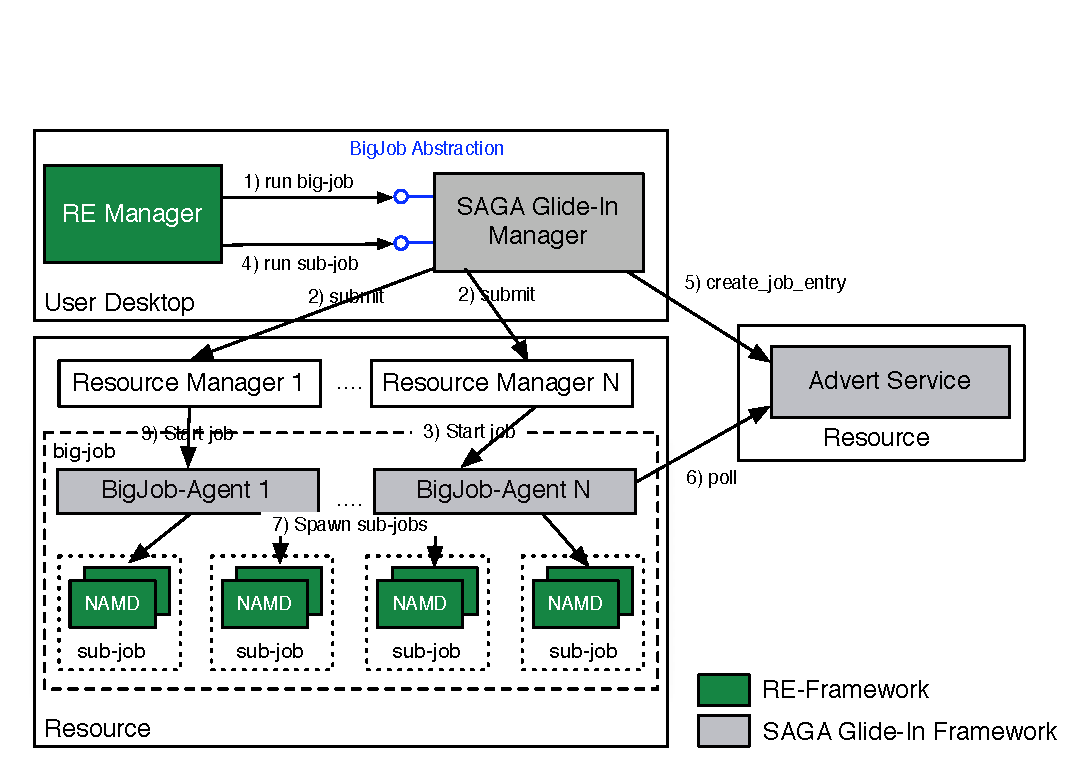
\includegraphics[width=0.82\textwidth]{../figures/Bigjob_arch.pdf}
          \caption{\footnotesize SAGA/BigJob Architecture
              }
      \label{fig:bigjob}
\end{figure}

We have demonstrated the usage of the SAGA-based Pilot-Job
framework~\citep{saga_bigjob_condor_cloud} -- called the BigJob, to
run RE simulations across multiple, heterogeneous, distributed grid
and cloud infrastructure~\citep{Luckow:2008fp}.  SAGA~\citep{saga-url}
is an API to the basic functionality required to build distributed
applications, tools and frameworks so as to be independent of the
details of the underlying infrastructure.  The various tasks that are
carried out using the SAGA APIs include file staging, job spawning and
the conduction of the exchange attempts.

Here we use the BigJob framework to efficiently request and manage
computational resources for multiple replicas.  Specifically, it
enables the dynamical utilisation a range of infrastructures, i.e., it
supports a scheme that does not depend on a static set of resources
that are pre-defined at the time of workload submission.

Figure ~\ref{fig:bigjob} shows the architecture of SAGA BigJob.  It
consists of three components: (i) the SAGA-BigJob Manager, (ii) the
BigJob Agent and (iii) the advert service which is a central key/value
store which is used for communication between the SAGA-BigJob Manager
and the BigJob agent.  The SAGA-BigJob manager submits the BigJobs to
the resource manager and sub-job descriptions to the advert server.
There is a separate BigJob agent for each BigJob, even if there are
multiple BigJobs on a given machine.  Once a BigJob becomes active,
the BigJob agent retrieves the job descriptions from the advert
server, allocates the required number of nodes and launches the
sub-jobs on each resource. The BigJob agent continuously monitors the
running sub-jobs and updates the sub-job states in the advert
server. Once a sub-job finishes running, the nodes are freed and
marked as available. The BigJob agent periodically polls the advert
server for new jobs.

\subsection{Replica-Exchange Manager}\label{repexmanager} 

% \jhanote{Abhinav: This subsection should help the reader understand
%   the basic and common elements of the RE Framework -- job submission,
%   role of bigjob-agent, replica agent, replica-exchange manager etc
%   etc} \athotanote{job submission, bigjob agent are explained in 3a. RE Manager is explained below. replica agent is touched upon but a more detailed explanation in section 3b(ii)}
  
%   \jhanote{ABHINAV: DEFINE THE ROLE OF RE-MANAGER HERE.  Possibly BIGJOB
%   AGENT here if not in previous subsection.}  \athotanote{please check if it's ok now}
  
The RE Manager is the master process controlling the different
components of the framework and aspects of the exchanges.  The RE
Manager % is an abstraction that
uses the SAGA BigJob Manager; the actual tasks that the RE Manager
performs out depend on which RE algorithm is being investigated.  A
replica agent is a wrapper script that manages an individual
replica  -- starts, facilitates the exchange of that replica,
and restarts it.

% And at the least, it is the SAGA BigJob Manager.  At the most,
% launched in place of the replica. The replica agent implementation
% where the RE Manager does a lot of work (a centralized
% implementation). But in an implementation where there is a
% \emph{replica agent} for every replica, the It should be noted that
% synchronous and asynchronous RE are different algorithms and the
% implementation of same algorithm could be centralized and
% decentralized.

The asynchronous RE algorithm can be implemented using a centralised
or decentralised coordination scheme.  In the former, the RE Manager
manages all the replicas and performs the exchanges; in the
decentralised coordination implementation, multiple replica-agents
take on that responsibility.  It is worth noting that the synchronous
RE algorithm has centralised coordination scheme.  Interestingly, for
decentralised coordination implementation, the RE Manager is
functionally similar to the SAGA BigJob Manager.

% Synchronous RE is implemented in a centralised fashion. Centralized
% implementation suits synchronous RE because there is a
% synchronization step at the beginning of each exchange step. But we
% implement asynchronous RE in both centralised and decentralised
% fashions.

% The RE-Manager also creates directories, configuration files and
% stages them to the respective directories.  \alnote{We should focus
%   on the RE part here. The BigJob stuff move to subsec a). This
%   should also remove the redundancy with a)}

\begin{figure}%
\centering
\subfigure[Central]{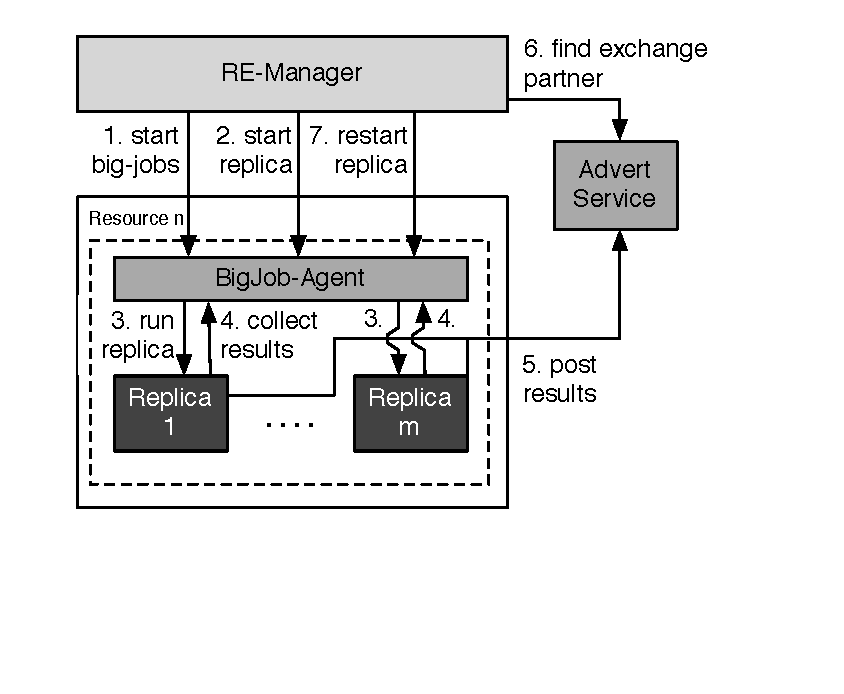
\includegraphics[width=0.47\textwidth]{../figures/central_AL.pdf}}\qquad
\subfigure[Decentral]{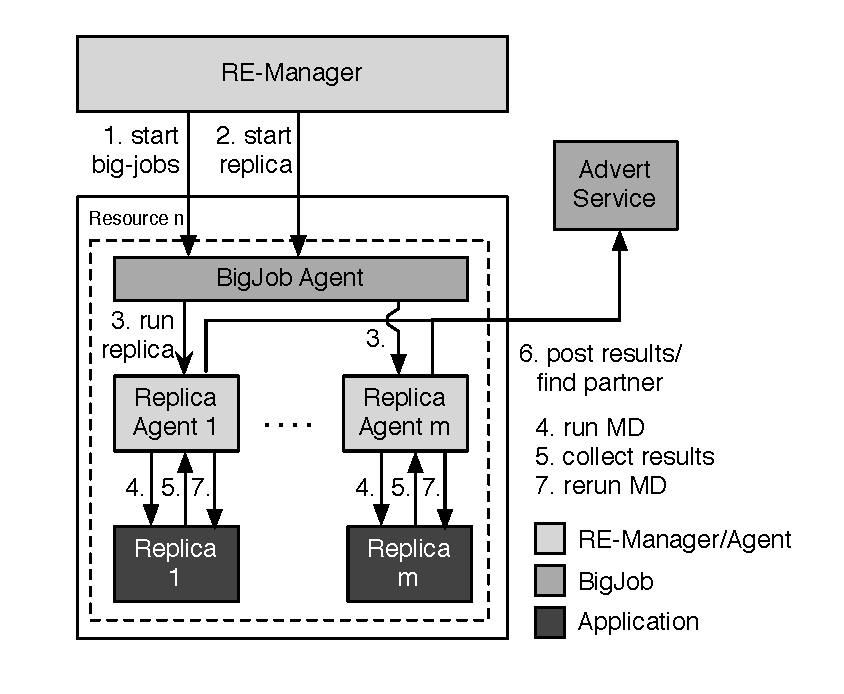
\includegraphics[width=0.47\textwidth]{../figures/decentral_AL.pdf}}\\
\caption{\textbf{Centralised vs. Decentralised Coordination:} Both
  central coordination style is used both by the synchronous RE (case
  I) and a version of the asynchronous RE (case II).  In the decentral
  style -- used by another version of the asynchronous RE (case III)--
  the master is only required for initially setting up all
  replicas. The later coordination is done peer-to-peer via the Advert
  Service.}
\label{fig:coordination}
\end{figure}

% \jhanote{this is an implementation detail. Abhinav: IIUC we restart in
%   both cases -- successful and unsuccessful exchanges. Non? ALso don't
%   toggle between ``replicas'' and ``jobs''!}  

We first explain how the synchronous and asynchronous (centralised) RE
Manager works in the following section followed by an explanation of
how the asynchronous (decentralised) RE Manager/replica agent
combination works.

\subsubsection{Synchronous and Asynchronous (centralised) RE-Manager}

% We first explain how the synchronous RE Manager works and then
% explain asynchronous (centralized) RE Manager. 
% centralized implementation, Figure~\ref{fig:coordination}a) can be
% used to describe both.

% The architecture of an asynchronous (centralized) RE-Manager is
% similar to that of synchronous RE Manager.
% Figure~\ref{fig:coordination}a) shows the control flow.

The control flow of a centralised RE scheme is shown in
Figure~\ref{fig:coordination}(a), which can be used to understand both
the asynchronous (centralised) RE and synchronous RE implementations.
Once the BigJobs and replicas are running, the RE Manager constantly
queries the SAGA BigJob Manager for the latest replica states.  When
the RE-Manager finds a replica that has finished running, it collects
the energy and temperature of that replica by reading the output
file. Once \emph{all} the replicas have finished running, the
RE-Manager makes the exchanges. The exchange is done by exchanging the
temperatures and writing new configuration files. The new
configuration files are staged to the appropriate location. The
RE-Manager then submits the replicas for restarting. % \alnote{The  RE-Manager spawns a new sub-job. BJ uses the advert service to  dispatch this subjob. See comments above} \jhanote{Needs fixing}
The SAGA BigJob Manager restarts them. The RE-Manager
counts the successful exchanges. This process is repeated until the
required number of exchanges are done.

The difference in the implementation of the asynchronous (centralised)
RE-Manager, is that instead of waiting for \emph{all} replicas to
finish running before making exchanges, whenever the asynchronous
(centralised) RE-Manager finds a replica that has finished running, it
tries to find a partner to make an exchange. In order to find a
partner, the RE Manager goes over the list of all the replicas in the
ensemble. If it finds a replica available it attempts the exchange. If
a replica is not found available, the RE Manager queries the SAGA
BigJob Manager for the latest replica states and updates its local
list. It then loops over the list to find a replica that has finished
running and a partner to exchange with that replica.  If successful,
the replicas are submitted to be
restarted. % \alnote{see comment about BJ
%   impl. detail above}.
The RE-Manager counts the successful
exchanges. This process is repeated till all the exchanges are made.


% \alnote{Not sure what we should do with the following paragraph}
% \jhanote{Does not belong here} It should be noted that where as in the
% synchronous RE, the exchanges are conducted when all replicas finish
% running. And the replicas are restarted only after all the exchanges
% are completed. But in an asynchronous (centralized) RE, the exchanges
% are conducted whenever possible and the replicas are restarted.

\subsubsection{Asynchronous (decentralised) RE-Manager and the replica agent}

% Thus, after the replica-agents are launched, the RE Manager and the
% SAGA BigJob Manager don't have any responsibilities.
 

Figure~\ref{fig:coordination}(b) shows the asynchronous (decentralised)
RE control-flow.  In the asynchronous (decentralised) implementation,
in order to conduct the exchanges the RE-Manager launches multiple
replica-agents (in lieu of replicas directly).  Replica-agents then
take control of replica start/re-start and exchange attempts.  The
replica-agents upon launch, run the replicas; the nodefile is passed
to the replica-agent as an argument at startup. The replica-agent
constantly monitors the replica, and when the replica finishes, it
updates the advert server with the current state of that replica.  It
also reads the temperature and energy from the output files, and posts
the values to the advert server.  The RE Manager is is primarily
responsible for keeping track and count of the number of exchanges
performed; when the desired number of exchanges are done, the RE
Manager ends the experiment.

% \jhanote{ISNT THE NEXT PARAGRAPH ESSENTIALLY THE SAME AS THE PREVIOUS
%   PARAGRAHGP? WHY DONT YOU REFER TO THE FIGURE AND THE BASIC StePS
%   OUTLINED IN THE FIGURE?}
  
% \begin{figure}[t] \centering
%           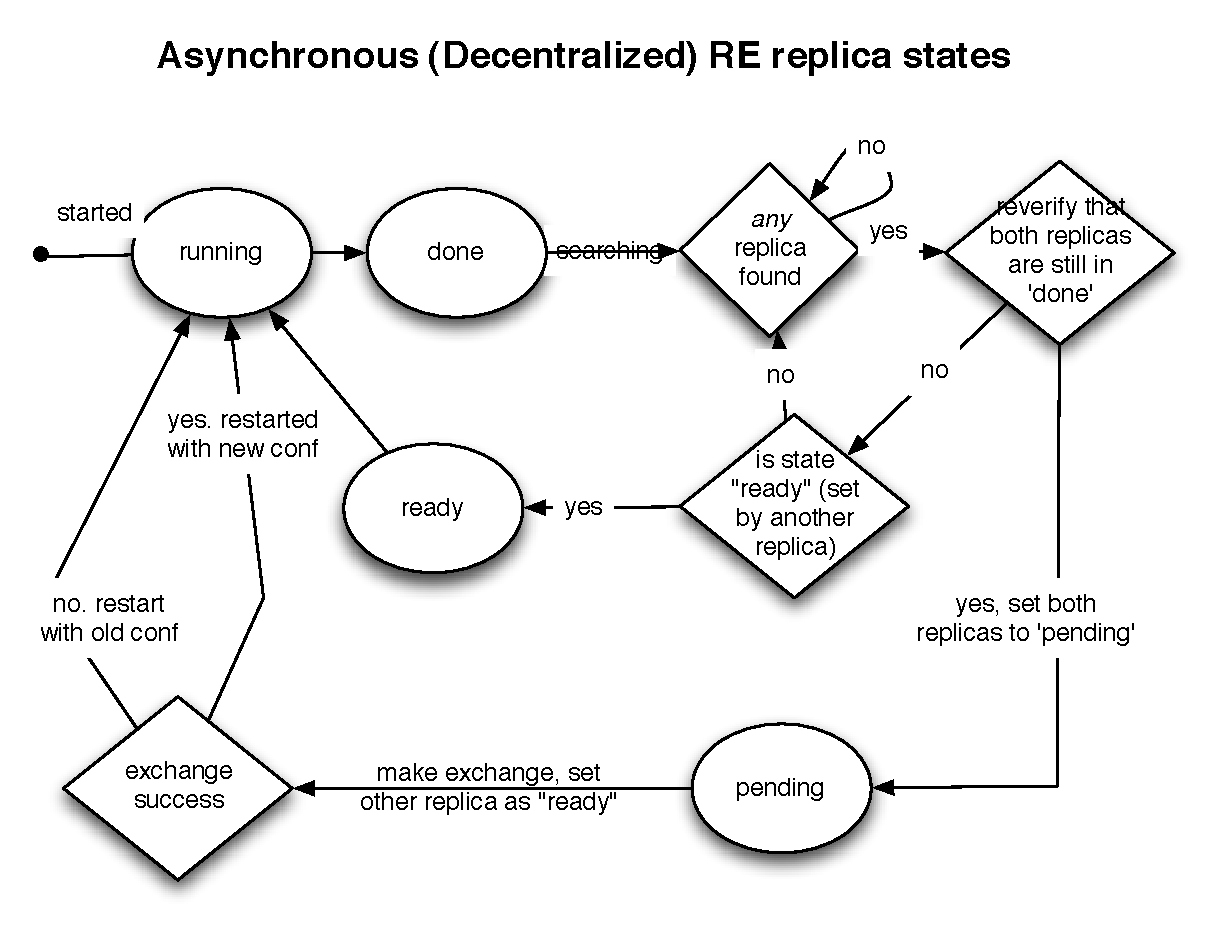
\includegraphics[width=0.82\textwidth]{../figures/decent_state.pdf}
%           \caption{\footnotesize Asynchronous (decentralized) RE
% replica state diagram } \alnote{This chart is not correct yet. There
% can't be state changes on conditional fields} \jhanote{is this a four
% state model or a 3 state model?}
%       \label{fig:state}
% \end{figure}

% As shown in state diagram  (Figure \ref{fig:state}) 
% The replica-agent also goes through the list of replicas randomly to
% try to find an exchange partner.  

\alnote{In the original state chart we had a ``free'' state. I think
  this state is needed to ensure the atomicity property of the
  exchange protocol (2pc style).} \jhanote{Would the \texttt{free}
  state the same as the \texttt{complete} state?} A replica can be in
one of the three states: (i) \texttt{running}, (ii) \texttt{done},
(iii) \texttt{pending} (for an exchange) and (iv) \texttt{complete}
(exchange has been completed). \athotanote{after an exchange is
  complete, the state has to be set as complete by the
  exchange-initiator, so that the other replica-agent can restart its
  replica} When a replica reaches a pre-determined state it (the
replica-agent acts as the proxy for the replica) transitions from
\texttt{running} to \texttt{done}. It initiates the search for a
partner.  (The search for an exchange partner is conducted in a random
manner so as to avoid having all the replicas starting at the first
replica, which causes contention and failed exchanges).  If a replica
finds another replica available, it reverifies their states (to ensure
that both replicas are still in \texttt{done} state) and sets their
states as \texttt{pending}. After making the exchange (changing the
temperature of both replicas in the advert server), it sets their
states as \texttt{complete}. Now both replica-agents write new
configuration files with the updated temperatures from the advert
server and restart their replicas.

To ensure atomicity of the state transitions, after the initiating
replica finds an exchange partner, it {\it reverifies} its state,
i.e., it has not been chosen by another partner in the duration that
it was finding a partner.  If the initiating replica's state has
changed, then the replica aborts the exchange process it initiated,
and waits for its state to be set to \texttt{complete}, so that it can
restart its replica. \jhanote{I don't understand how its state is set
  to complete and then to restart the replica}.  The replica
\jhanote{Do you mean replica-agent?} that initiated the exchange
increments the exchange count. The RE Manager constantly queries the
advert server for the latest exchange count and when all exchanges
have been made, it stops the experiment.

% At the point where the first replica reverifies the states, if one of
% the replicas' states have changed: (i) if it is the second replica,
% the replica agent tries to find a new replica; (ii) if it is the first
% replica itself, that would mean another replica has set the replica as
% \texttt{pending}. 

\subsubsection*{This paragraph to be removed on discussion}

% , it re-verifies the
% states of both itself and the other replica and if both are still
% available, 
% exchanges their temperature values on the advert server.  

% \jhanote{I though the RE-Manager did the following} \athotanote{the
%   replica agent increments the count, the RE Manager gets the count
%   from the advert server. Please look at the above para and tell me it
%   makes sense}\jhanote{OK. thanks}

\jhanote{I don't understand any of the stuff below. State changes have
  to be atomic!?: If the state of any of the replicas negotiating the
  exchange changes at the time of re-verifying the replica pair's
  states, that would mean that one or both of the replicas' is now in
  the process of making an exchange with a different replica. In that
  case one or both of the replica agents will wait till their state is
  set as "Ready" and start their next run. If one of the replicas is
  still available, it tries to find a new partner for exchange.}
\athotanote{i was trying to say the following: replca 1 finds replica
  2 in done state, but before it locks replica 2, it reverifies both
  states. (replica 1, while searching could have been set to pending
  by replica x) If states are still done, the replicas are locked and
  exchange is made. I made some changes in the explanation. please see
  if its easier to understand now.}\jhanote{Lets talk about this. I
  don't think another replica should be allowed to change the state
  of the ``initiating'' replica whilst the ``initiating'' replica
  is out looking for a partner}

% The search for an exchange partner is conducted in a random manner so
% as to avoid having all the replicas starting at the first replica,
% which causes contention and failed exchanges. If it finds another
% replica available, it re-verifies the states of both itself and the
% other replica and if it finds both still available, marks their states
% as "Pending". Let the replica initiating the exchange be $R_a$ and the
% other replica be $R_b$.  The replica $R_a$ which initiates the
% exchange is the replica in-charge of the exchange. $R_a$ then
% exchanges their temperature values on the advert server.  \alnote{We
%   should detail the exchange protocol. How do we ensure that the
%   exchange is atomic? figure?}  It then modifies its configuration
% files locally, sets its state as running and runs the replica. On the
% other hand, the $R_b$'s state is set as "Ready" by $R_a$ and that
% makes the $R_b$'s replica agent to retrieve its own temperature
% (modified by the $R_a$) from the advert server, modify its
% configuration file locally and run the replica. \alnote{Why does it
%   need to modify its own config if it uses its own temperature?}
% \athotanote{fixed} This removes the need to stage the configuration
% files to different machines. This is possible because there is a
% replica agent for each replica locally. Where as earlier, the
% RE-Manager and the replica might be located on different machines.  If
% the state of any of the replicas negotiating the exchange changes at
% the time of re-verifying the replica pair's states, that would mean
% that one or both of the replicas' is now in the process of making an
% exchange with a different replica. In that case one or both of the
% replica agents will wait till their state is set as "Ready" and start
% their next run. If one of the replicas is still available, it tries to
% find a new partner for exchange.  \alnote{How often is the process
%   repeated until the replica is started with the old temperature?}
% \athotanote{fixed}The replica agent that initiated the exchange
% increments the exchange count by one.  If an exchange fails due to
% contention, the replica agent tries to find a new partner. If an
% exchange is deemed unsuccessful after comparison of energies or
% temperatures, the replicas are restarted with their old
% configurations.

% \jhanote{Do we have a pending state? Accoridng to Abhinav there is
%   only a two-state model -- run and done?!} 
% \athotanote{should i keep the state diagram? do you suggest any
%   corrections to the state diagram? i also think that instead of
%   having the current control flows, we should have figures showing how
%   the exchanges are made or instead hae state diagrams. the control
%   flows right now show a lot of stuff already shown in the bigjob
%   architecture figure. }
  

\section{Implementation of Synchronous and Asynchronous RE}
\label{sec:re_impl}
% \jhanote{This section should help the reader understand the control
%   flow - which is YOUR IMPLEMENTATION of the RE algorithm. Need to
%   make reference to Figures 2a and 2b} \athotanote{i think we are doing this in section 3?}\jhanote{Yes}

% \alnote{General remark: What do you guys think of summarizing the data into 
% a table? This way the reader can track the numbers at one central place.}
% \jhanote{YES. I have suggested the same too}


% \jhanote{Explain centralized and decentralized} \alnote{The question
%   is: where do we explain it? There are already a lot of details in
%   sec III}\jhanote{Yes. Old remark. Will be removed}


\begin{table}
    \centering
	\begin{tabular}{|l|c|c|c|}
	\hline
	                        &synchronous  &asynchronous-centralised &asynchronous-decentralised\\
	% \hline
	%  $T_{MD\_init}$  &23\,sec &23\,sec &23\,sec\\
	%  \hline
	%  $T_{MD\_run}$   &68\,sec &68\,sec &68\,sec\\
	\hline
	$T_{MD}$       &71\,sec &71\,sec &71\,sec\\
	\hline
	\hline
	$T_{W}$        &2.64\,sec &1.02\,sec &2.03\,sec\alnote{todo discuss!}\\
	\hline
	\hline
	$T_{X}$        &0.62\,sec &0.78\,sec &2.29\,sec\\
	\hline
	\hspace{2mm}$T_{F}$        &0\,sec   &0.16\,sec &1.65\,sec \alnote{we need to analyze this mis-match}\\
	\hline
	\hspace{2mm}$T_{EX}$       &0.4\,sec &0.4\,sec &0.64\,sec???\\
	\hline
    \hspace{2mm}$T_{COORD}$    &0.22\,sec &0.22\,sec    &NA (included in $T_W$)\,\\
	\hline
	\hline
	$\mathbf{T_{C}}$        &\textbf{990\,sec} &\textbf{798\,sec}    &\textbf{603\,sec}\\
	\hline
    \end{tabular}
	\caption{Replica-Exchange Performance}
	\label{table:repex_perf}
\end{table}

\alnote{Do we want to present impl. details here?} \athotanote{i too think that we are explaining how we implemented in section 3(RE Framework). Here we are analyzing our implementation?}
In this section we present the implementation of the different RE scenarios. 
Further, we analyse the primary components that impact the performance of a RE
simulation.  For this purpose the following configuration is used:
Nanoscale molecular dynamics (NAMD)~\citep{Phillips:2005gd}, a highly
scalable, parallel MD code, is utilised to carry out the MD simulation
corresponding to each replica run. It is important to mention that any
other MD or Monte Carlo code could be used just as simply and
effectively. The total number of replicas ($N_R$) in the ensemble are
32 and the total number of pairwise exchanges ($N_X$) is 128. As the
ensemble of replicas are run concurrently, 16 pairwise exchanges are
possible after each concurrent run. Thus, each replica on average is
restarted 7 times.  Our experiments are performed on LONI and Teragrid
shared resource \emph{QueenBee (QB)}. Each replica is configured to run 500
time-steps and is allocated 16 processors. It should be noted that we
are talking about the average values whenever we mention
quantities. % Each replica takes 91 seconds to complete the
% 500 time-steps from a fresh start and 68 seconds every time it is
% restarted. Thus, if each replica is restarted 7 times, the average
% time to complete 500 time-steps ($T_{MD}$) is ${(91+68\times 7) \over8} =
On average each 500 time-step run takes $71$ seconds. 
%\alnote{The 71\,sec average won't hold for larger $N_{x}$}
It should be noted that the replicas take longer (91 seconds) to
complete their 500 time-steps from a fresh start. But when they are
restarted, they finish the run slightly faster (68 seconds).  And the
total time the ensemble of replicas spend running is $71 \times 8 =
568$ seconds.
  
For all implementations, in the event of a successful exchange, jobs
are restarted~\citep{Luckow:2008fp} with new temperature values.  In
the case of an unsuccessful exchange, jobs are restarted without
exchanging the configuration.
 
Also, we are primarily interested in learning the scale-up and
scale-out properties of synchronous and asynchronous RE and hence are
not concerned by the queue wait time. Therefore, we only start
measuring when the BigJob agent starts running the replicas. Because,
almost every time, the RE Manager completes submitting the replicas
before the BigJob becomes active.

\subsection{Synchronous RE}
\label{sec:impl_sync_re}
% The replicas are run by the BigJob agent after the BigJob becomes
% active. The average time the Bigjob agent takes to start one replica
% is 0.3 seconds.  \alnote{Is this the time agent only? Or does it
%   include the submission time on the master?}  \athotanote{fixed in
%   last lines of the previous section. the time the master takes to
%   submit the replicas is being included in $T_EX$. The time spent at
%   BigJob agent is included in $T_W$. }  \alnote{Don't see any
%   reference to $T_{EX}$ in last section. Later you refer to the
%   resubmission time as $T_{coord}$. Also, I don't see this component
%   in the $T_W$ formula below. The reader will not know what to do with
%   the 0.6 sec!}  For a pair of replicas, it is 0.6 seconds.

The BigJob agent takes 0.92 seconds to process a replica that
has completed running.  That is the time it takes to update the state and
mark the nodes as free. Since the whole ensemble of replicas need to complete running, it is
sufficient to consider the longer of the time to start and the time to
mark the end of a replica run. Therefore, $T_r$ is included in $T_w$. The time spent waiting for all replica to complete running is $0.92\times32=29.44$ seconds. For a pair of replicas, $T_w$ is 29.44/16=1.84 seconds. The RE-Manager constantly queries
the advert server for the latest replica states and marks the replicas
which finish running as done and retrieves the current energies and
temperatures by reading the output files. Thus, the associated cost is 0.4 seconds per
replica and 0.8 seconds for a pair. Thus, $T_W$ = 1.84+0.8=2.64 seconds.  \alnote{What is the component that
  is actually spent waiting for the other replicas to complete. The
  times you mention above are times for actually doing something, but
  not waiting times!} \athotanote{is it better now?}

Since all the replicas finish running before the exchanges are
started, the RE manager won't spend any time searching for partners
and $T_F$ is 0 seconds. $T_{ex}$ includes updating configuration files
and transferring the them to their respective directories, in this
case, locally. It takes 0.2 seconds to write and copy a file
locally. $T_{ex} = 0.2 \times 2=0.4$ seconds. $T_{coord}$ is the time
required by the RE-Manager to resubmit the pair of replicas for restarting. On average $T_{coord}$ amounts to $0.11\,sec \times 2 =
0.22\,sec$. Therefore, $T_{X}$ is $0+0.4+0.22=0.62$ seconds.
% \alnote{We need to decide whether we use capital letters or not:
%   $T_{ex}$ vs. $T_{EX}$}
Substituting the above values in equation~\ref{eq:totaltime}, we get
\begin{eqnarray}
  T=  {1 \over p} \times {[ {(71\times {128\over 16}})+ (0.62 + 2.64)\times 128]} = {1 \over p} \times (990)
\label{eq:sync}
\end{eqnarray}
%\alnote{$T_{MD}$ should be also x Nx?}


\subsection{Asynchronous (centralised) RE}
% \alnote{please don't just copy paste. Only focus on the differences}

%As before, the average time the BigJob agent takes to
%start one replica is 0.3 seconds. For 32 replicas, it is 9.6
%seconds. Thus, the BigJob agent finishes starting the last replica before the a replica completes its run. 

%The BigJob agent
%would be ready to restart the replicas by the time the RE-Manager
%submits to the advert server. %\alnote{Not consistent with a) Where is the 71s number?}

As mentioned earlier, the BigJob agent takes 0.92 seconds to find that
a replica is done, update the state and free the nodes. But in this
implementation, we also make the BigJob agent also retrieve the energy
and temperature from the output files, which adds 0.2 seconds per
replica. In summary it takes 1.12 $\times$ 32 = 35.84 seconds for 32
replicas. As soon as the first pair of replicas are marked as done by the
BigJob agent, the RE-Manager makes the exchange between
that pair of replicas - and that pair of replicas would wait 32.8 seconds ($35.84-1.12\times2-T_X$) before the BigJob agent is able to restart
them. It can be seen from this equation that later pairs of replicas wait a smaller amount of time before they are restarted by the BigJob agent (the BigJob agent alternates between starting all replicas that are new and ending all replicas that are done). On average, this group (16 pairs) of replicas waits  32.8/2=16.4 seconds. Or each pair waited ($T_r$) 16.4/16=1.02 seconds.  \alnote{I don't understand the notion of pair in this context. Is 32 sec == $T_W$?}\athotanote{is it better now?} It should be noted that the timelines
of the RE-Manager and the BigJob agent run concurrently. Also, the time RE Manager waits for the next replica to become available, $T_w$ is included in $T_F$. Thus $T_W$ is 1.02 seconds.

The time the RE Manager takes to find a partner ($T_F$) depends on
$N_R$ and also on the number of replicas the RE-Manager has to sift
through to finds an available replica. On average, RE-Manager will
sift through $N_R/2$ replicas before it finds a partner. % \alnote{I
%   think this conflicts with the ```deterministic'' approach we
%   discussed yesterday}
It should be noted that we also implemented a
special case for an ensemble containing a very large number of
replicas, where the RE-Manager tries to find a partner randomly. We
observed that this only improves the performance when the ensemble
contains more than 128 replicas. It takes 0.01 seconds per
query to advert server. \alnote{Is this a remote query to the advert service?} \athotanote{yes}  If the RE Manager tries to find a partner for exchange in a linear fashion, it would have to go through 0 to 32 replicas. On average, it would go through 16 replicas to find a partner. $T_F$ is $16\times
0.01=0.16\,sec$. \alnote{i.e. per average 16 queries are necessary in
  order to find a partner? Why 16?} \athotanote{explained} $T_{ex}$ is the time it takes to
update the configuration files and copy them locally. That would be
$({0.2})\times 2=0.4\,sec$. $T_{coord}$ is the time it takes to
resubmit the pair of replicas to the advert server, which is
$0.11\times 2 = 0.22$ seconds. Therefore, $T_{X}$ is
$0.16+0.4+0.22=0.78$ seconds. 

% The point we are trying to make is that the BigJob agent might not
% be free while the RE-Manager submits the replicas to be
% restarted. But as the experiment progresses, instead of all the
% replicas in the ensemble running in synchronization, pairs of
% replicas would start and end together.  By the time the BigJob agent
% finishes processing the last of the replicas that finished running,
% the RE-Manager would have re-submitted 15 pairs of replicas to the
% advert server for restarting by the BigJob agent. In the next couple
% of seconds the rest of the replicas would have been exchanged and
% submitted to the advert server.


Substituting the above values in equation ~\ref{eq:totaltime}, we get:
\begin{eqnarray}
T=  {1 \over p} \times {[ {(71\times {128\over 16}}) + (0.78 + 1.02)\times 128]} = {1 \over p} \times 798.4 seconds
\label{eq:cent}
\end{eqnarray}


\subsection{Asynchronous (decentralised) RE}

\athotanote{we can remove the sentence about 0.3/10 seconds, what do you think?}When the BigJob becomes active, the BigJob agent starts the replica
agents and the replica agents in turn start the replicas. It takes 0.3
seconds to start a replica-agent (but this is only a one time event and does not influence the overall time to completion by more than 10 seconds). The replica agent creates the
output and error files, reads the configuration, opens a connection to the advert server, sets the state to running and starts the
replica. All these actions, which are repeated after every exchange,
take ($T_r$) 1.3 seconds. \alnote{How do you get 1.3 sec? The starting of the replica-agent
must not be repeated after every exchange, correct?} \athotanote{fixed. is it ok now?}

The replica agent constantly monitors all replicas. If it finds
a replica that completed its run, it updates its state in the advert
server, which takes 0.11 seconds \alnote{A advert modification took in the previous
cases 0.01\,sec? What is different here?}.\athotanote{yes, the number of connections to the advert server effects the performance} Also, it retrieves the energy and
temperature from the output files, each of which actions take 0.2
seconds. It then posts both these values to the advert server. These are the associated costs: $0.11+0.2\times2+0.11\times2=0.73$ seconds.  Thus,
$T_W$ is 1.3 + 0.73=2.03 seconds.\alnote{Where is the 0.7 sec coming from?} \athotanote{fixed. is it okay?}

We observed that on average, the replica agent makes 15 random queries before
it locks a partner to make the exchange. \alnote{Why 15? Previously, it has been 16.} \athotanote{random queries}
Each query is 0.11 seconds, thus $T_F$ is 1.65
seconds. The process of changing the states
and temperatures in the advert server and writing a new
configuration file takes, $T_{ex} = 0.11\times 4 +0.2 = 0.64$ seconds.
\alnote{What is the difference between $T_F$ and $T_{ex}$ here?} 
(And even in the other scenario, where the replica in question is not the
initiator of the exchange, it has to wait for the other replica to set its state as complete, so that it can restart.) $T_{coord}$ is the time it takes to
update the state in the advert server, which is included in $T_r$. \alnote{In the other
cases the state must be updated in the advert server as well. Why don't we consider
this in the other cases as well?}\athotanote{in the other two cases, the bigjob agent makes the state changes} Thus,
$T_{X}$ is $1.65+0.64= 2.29$ seconds.

It should be noted here that in the centralised version of
asynchronous RE, where only 2 connections to the advert server existed
(RE-Manager, BigJob agent), each query took only 0.01 seconds. But in
the decentralised version, since each replica agent maintains an open
connection to the advert server, there are 32+2=34 connections
open. This effects the performance of the advert server. This is the reason we find that each query is 0.01 seconds in the centralised implementation and 0.11 seconds in the decentralised implementations. \alnote{Is this the reason why
the query takes 0.11\,sec instead of 0.01\,sec now? These would be a severe performance
degradation.}

\athotanote{ do we need this para?}In the decentralised implementation, there are many pairs of
replica agents negotiating the exchanges concurrently. While this
causes the time taken per unit exchange to go up, more exchanges occur
in unit time.

Substituting the above values in equation~\ref{eq:totaltime}, we get:
\begin{eqnarray}
T=  {1 \over p} \times {{(71\times {128\over 16}}) + {(2.29+2.03)\times 128\over 16}} = {1 \over p} \times 603 seconds
\label{eq:decent}
\end{eqnarray}


%\alnote {one could ask why is the config file staged in case I and II then?} 

% \begin{figure}
% \centering
% %\subfigure[Control Flow: Decentralized Replica Exchange]{
% 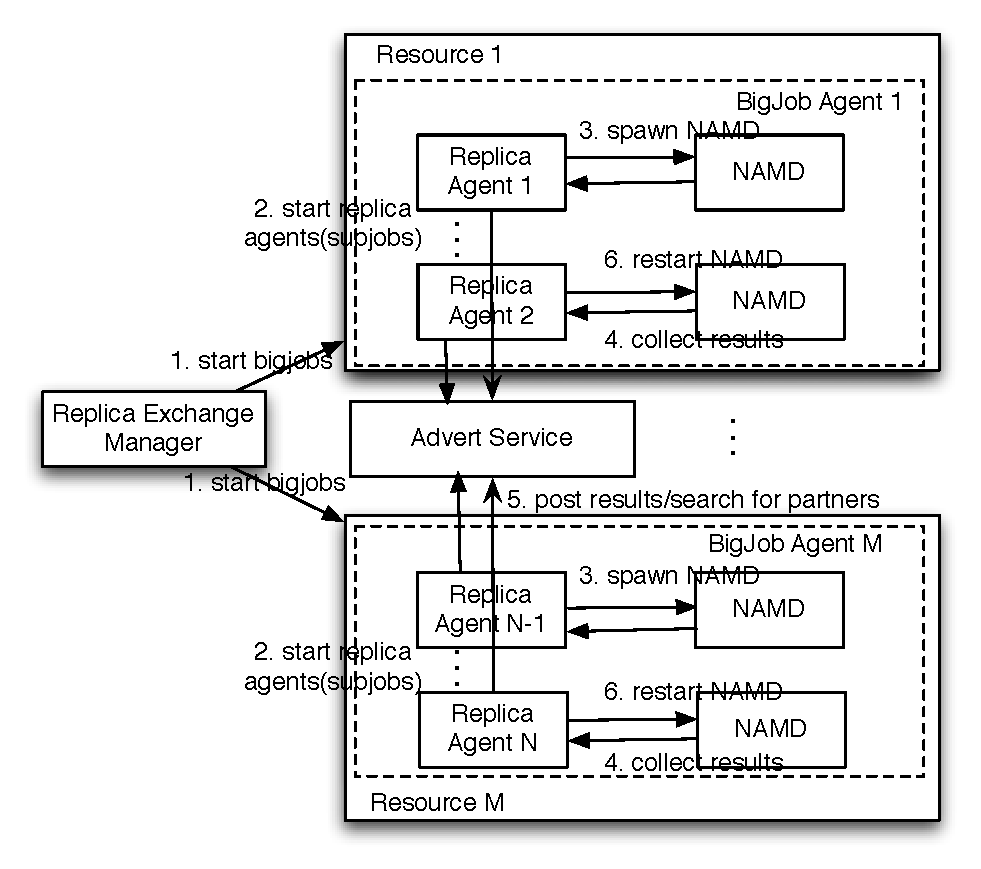
\includegraphics[width=0.9\textwidth]{asyncre.pdf}
% %\label{fig:async:b}
% \caption{\small Decentralized control flow: In the decentralized asynchronous RE, for  each replica there is a replica agent which individually manages the replica.}
% \label{fig:decent}
% %\vspace{-1em}
% \end{figure}

\alnote{we should write Case consistently with small or capital letter}
% We have to bear in mind that while Case II and Case III both implement the same asynchronous RE algorithm, they do it differently.
% At first glance it appears to be a question of philosophy, whether to
% let the replicas be managed by a master or to let each replica be
% managed individually.
%There could be implications effecting the performance of the
%algorithm. Where as in Case II, the master has to manage all the
%replicas and since it can only manage one replica at a time, although negligible, it is a cause for concern with large number of replicas. %The effect could be negligible and might now effect the overall performance.
%But the decentralized version (Case III) has no
%such issues as each replica is managed individually. % \jhanote{The distinction between Case 3 and 2 needs to
%  be made more clear. The following is ``implementation detail''. What
%  is the conceptual difference between Case 3 and Case 2?}

\section{Scale-Up and Scale-Out: Experiments and Results}
\label{sec:performance}

To evaluate the performance of the different RE implementations, several 
experiments have been conducted on TG and LONI resources. In particular, 
we investigate the performance of the three RE implementations -- synchronous (case I),
asynchronous-centralised (case~II) and asynchronous-decentralised (case III) -- with
respect to different number of replicas and machine configurations.
While in the ``scale-up'' scenario a single machine is used, in the ``scale-out''
scenario up a RE simulation is carried out on up to 4 machines concurrently.
As in the previous analysis we use NAMD to carry out MD simulations. Each
replica uses 16 MPI processes and runs 500 time steps. A temperature range 
between 300 and 3000 K is sampled.
\alnote{Should we reference the model used? Not sure which model it is
Hepatitis or HIV?}

% One set of experiments are modeled to 
% analyze the performance of the algorithms and implementations when we 
% increase the number of replicas while keeping the number of machines 
% a constant. The other set of experiments are modeled to analyze the 
% performance when the number of replicas is kept a constant but the 
% number of machines is increased. We call the former "scale-up" and 
% the latter "scale-out" scenario.

%
%%%%% FIGURE %%%%%
\begin{figure}
\centering
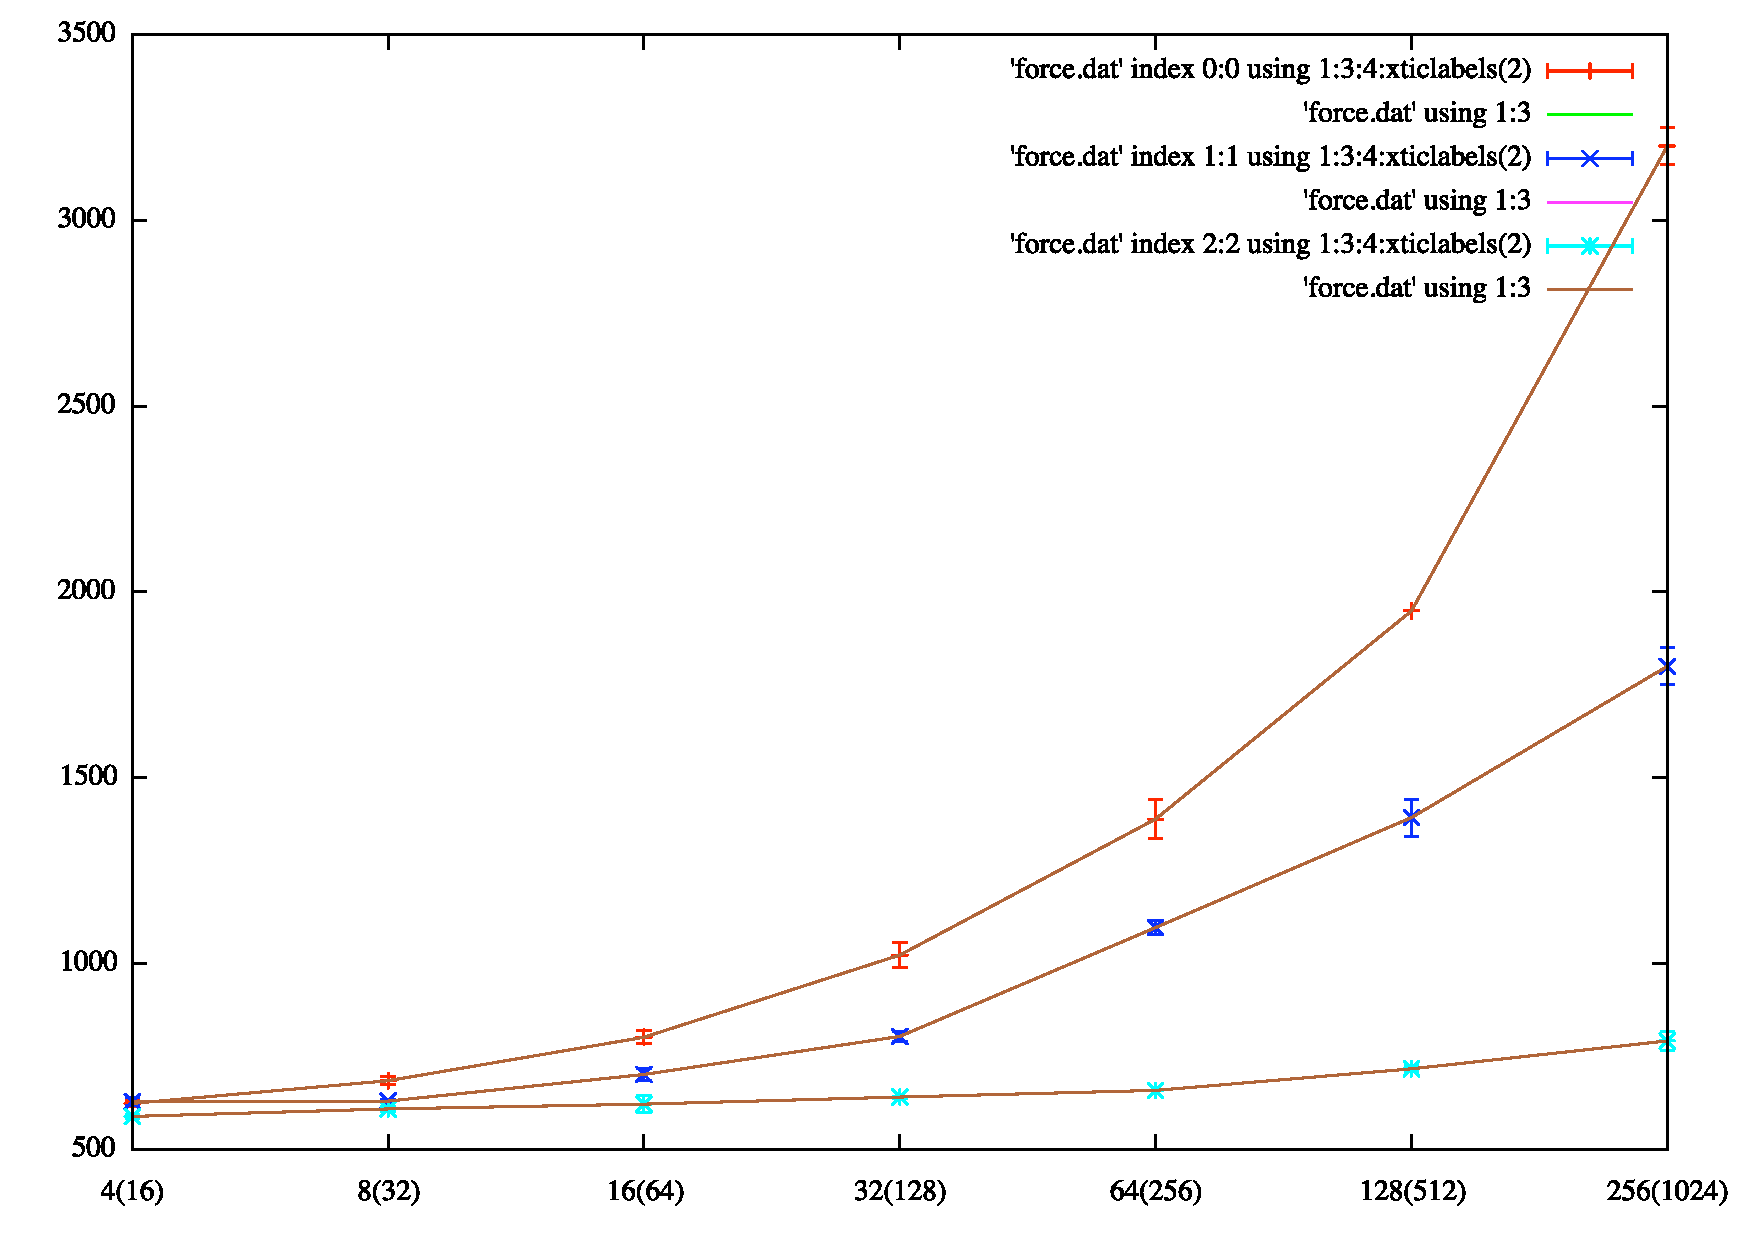
\includegraphics[width=0.9\textwidth]{../data/scale_up_gnu.pdf}
\caption{\small \textbf{Scale-Up Performance for 8 to 256 Replicas:} 
  The graph shows the runtimes for the different RE implementations.
  The asynchronous decentralised RE implementation shows the best
  scaling behaviour. Both centralised RE versions scale less well mainly due
  to the limitations of the single master, which becomes a bottleneck.}
\label{fig:graph}
\vspace{-1em}
\end{figure}

\subsection{Scale-Up}

{\it Experiments: }
In this scenario we run the defined RE configuration using the three RE implementations 
and between 4 and 256 replicas on the Teragrid resources QB and Ranger.
Both resources deliver a comparable performance; QB however has a maximum
core limit of 2048 cores per jobs. For all runs, a single BigJob with a 
sufficient number of cores is used. 
% Up to 128 replicas, all simulations were conducted on
% QueenBee, but the 256 replica simulations were conducted on Ranger as
% QueenBee allocates a maximum of 2048 cores per job. 
We measure the time-to-completion $T_{C}$ for four 
exchange attempts per replica, i.\,e.\ for 4 replicas $T_{C}$
for 16 attempts, for 8 replicas $T_{C}$ for 32 attempts,
etc., is measured. The ratio between the number of
replicas and attempted exchanges is kept constant, for
the purpose of comparison between each of these cases. Further,
we do not consider the initial queuing time for the BigJob.

% It means that
% we are keeping the number of times each replica restarts,
% approximately, a constant.
% The metric used
% for comparison of 4, 8, 16, 32, 64, 128 and 256 replicas is the time
% to complete 16, 32, 64, 128, 256, 512 and 1024 attempted exchanges,
% respectively. \alnote{This is a little confusing. In the model we talk
% about successful exchanges all the time. Opinions?} 
% The mean runtime is obtained by subtracting the queue wait time of
% the BigJob from the total time. As the ratio between the number of
% replicas and number of exchanges is kept constant, ideally, the
% runtime must remain constant too. 

%\subsubsection{Scale up performance: Results and Analysis}

{\it Results:} Figure~\ref{fig:graph} shows the results of this 
experiment. As the number of replicas increases, $T_{C}$ increases 
as well. This increase, however, is not uniform across the three cases. 
We see the most slow down in case I and the least in case III.

\alnote{need to be aligned with sec 4}
{\it Analysis: } The synchronous version (case I) shows the
worst scaling behaviour due to various reasons: as described in section~\ref{sec:impl_sync_re},
$T_{W}$, i.\,e.\ the time spent waiting for other replicas of a generation to finish,
is the main driver of this performance degradation. Since replicas are currently started
sequentially by the master, a delay between the start and thus the termination of the first and 
last replica exists. Further, different nodes of a machine tend to show a slightly 
different performance. With more replicas, the time to start the replicas as well as the
synchronization time increases.  In case II, exchanges happen in
an asynchronous manner, but they are still orchestrated by the master. 
As the number of replicas increases, the master quickly becomes
a bottleneck. But in case III, the exchanges are all carried out in a
decentralised way, i.\,e.\ exchanges can occur concurrently between 
different pairs of replicas. Therefore, it can be concluded that the asynchronous
RE algorithm scales better and that the decentralised implementation
is superior to the centralised one.

%
%%%%% FIGURE %%%%%
\begin{figure}%
\centering
\subfigure[8 replicas]{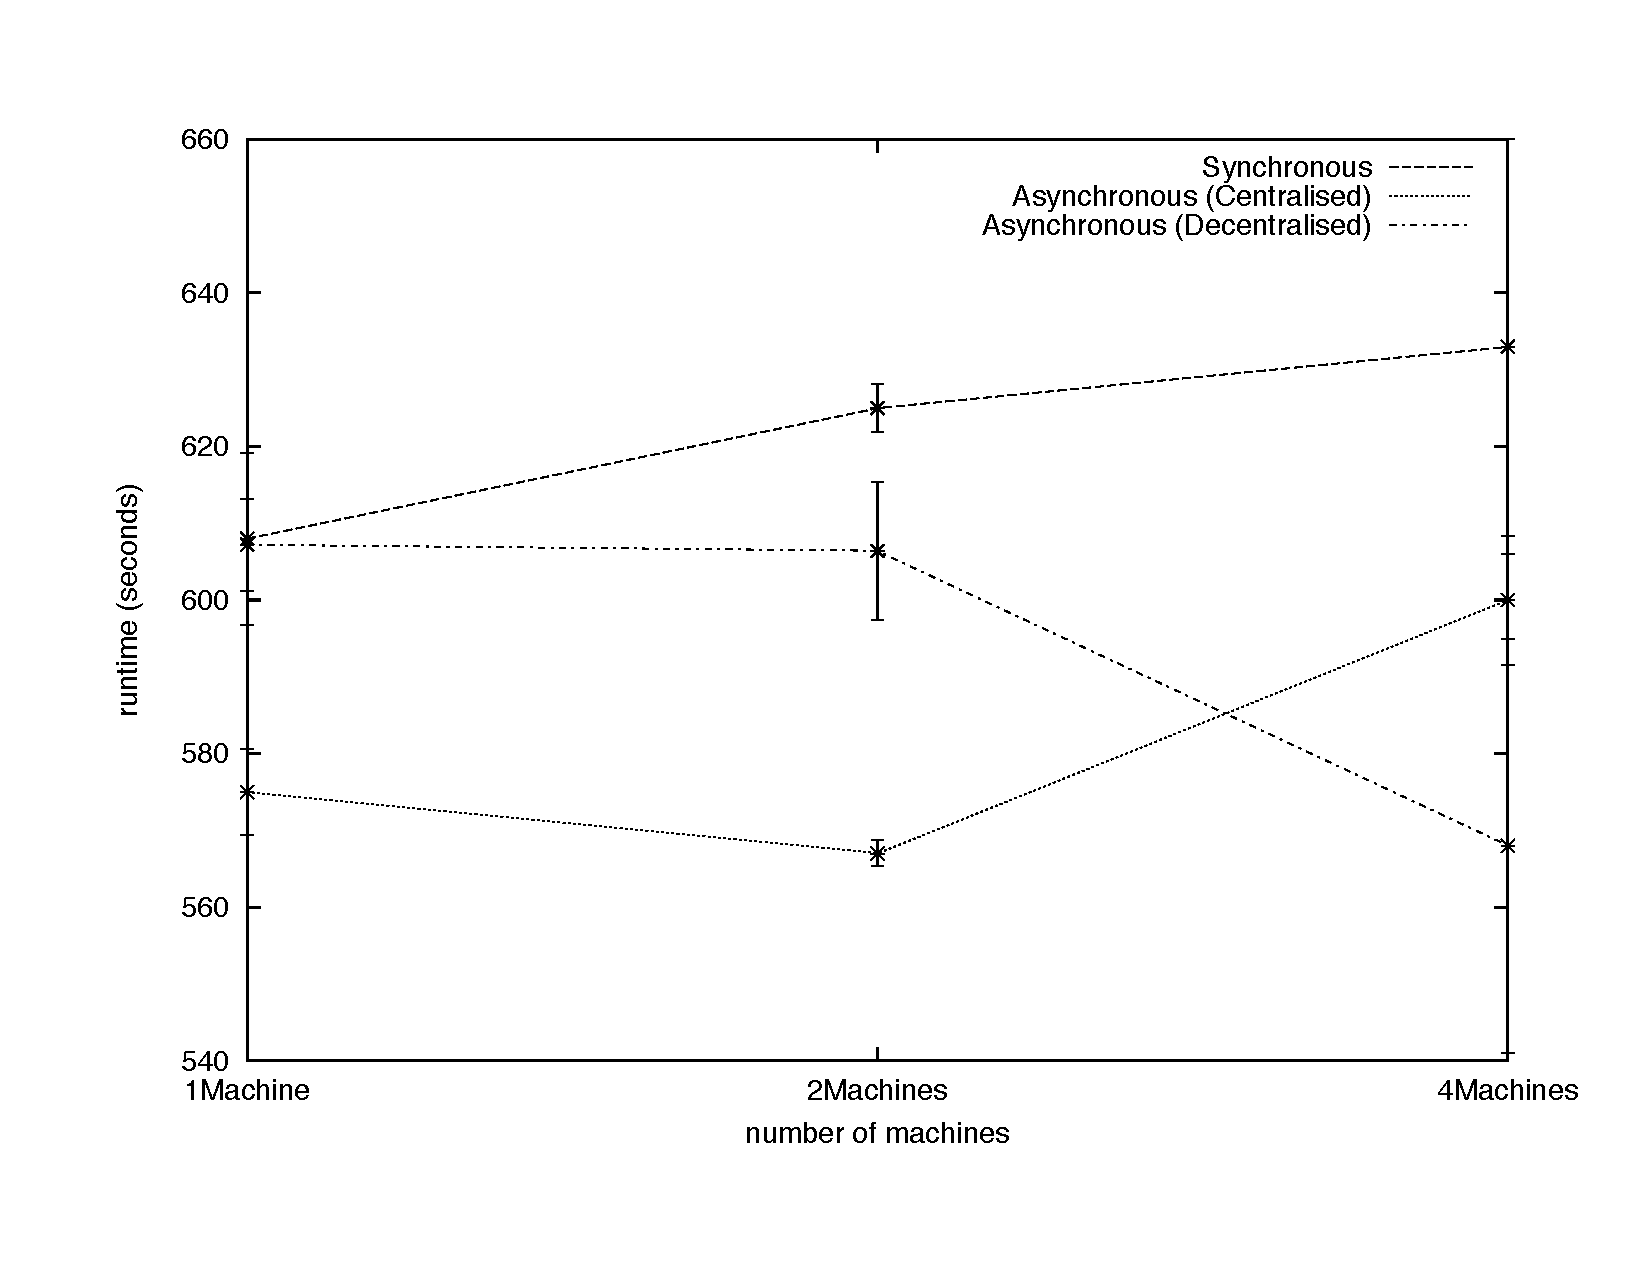
\includegraphics[width=0.47\textwidth]{../data/scaleo_8.pdf}}\qquad
\subfigure[16 replicas]{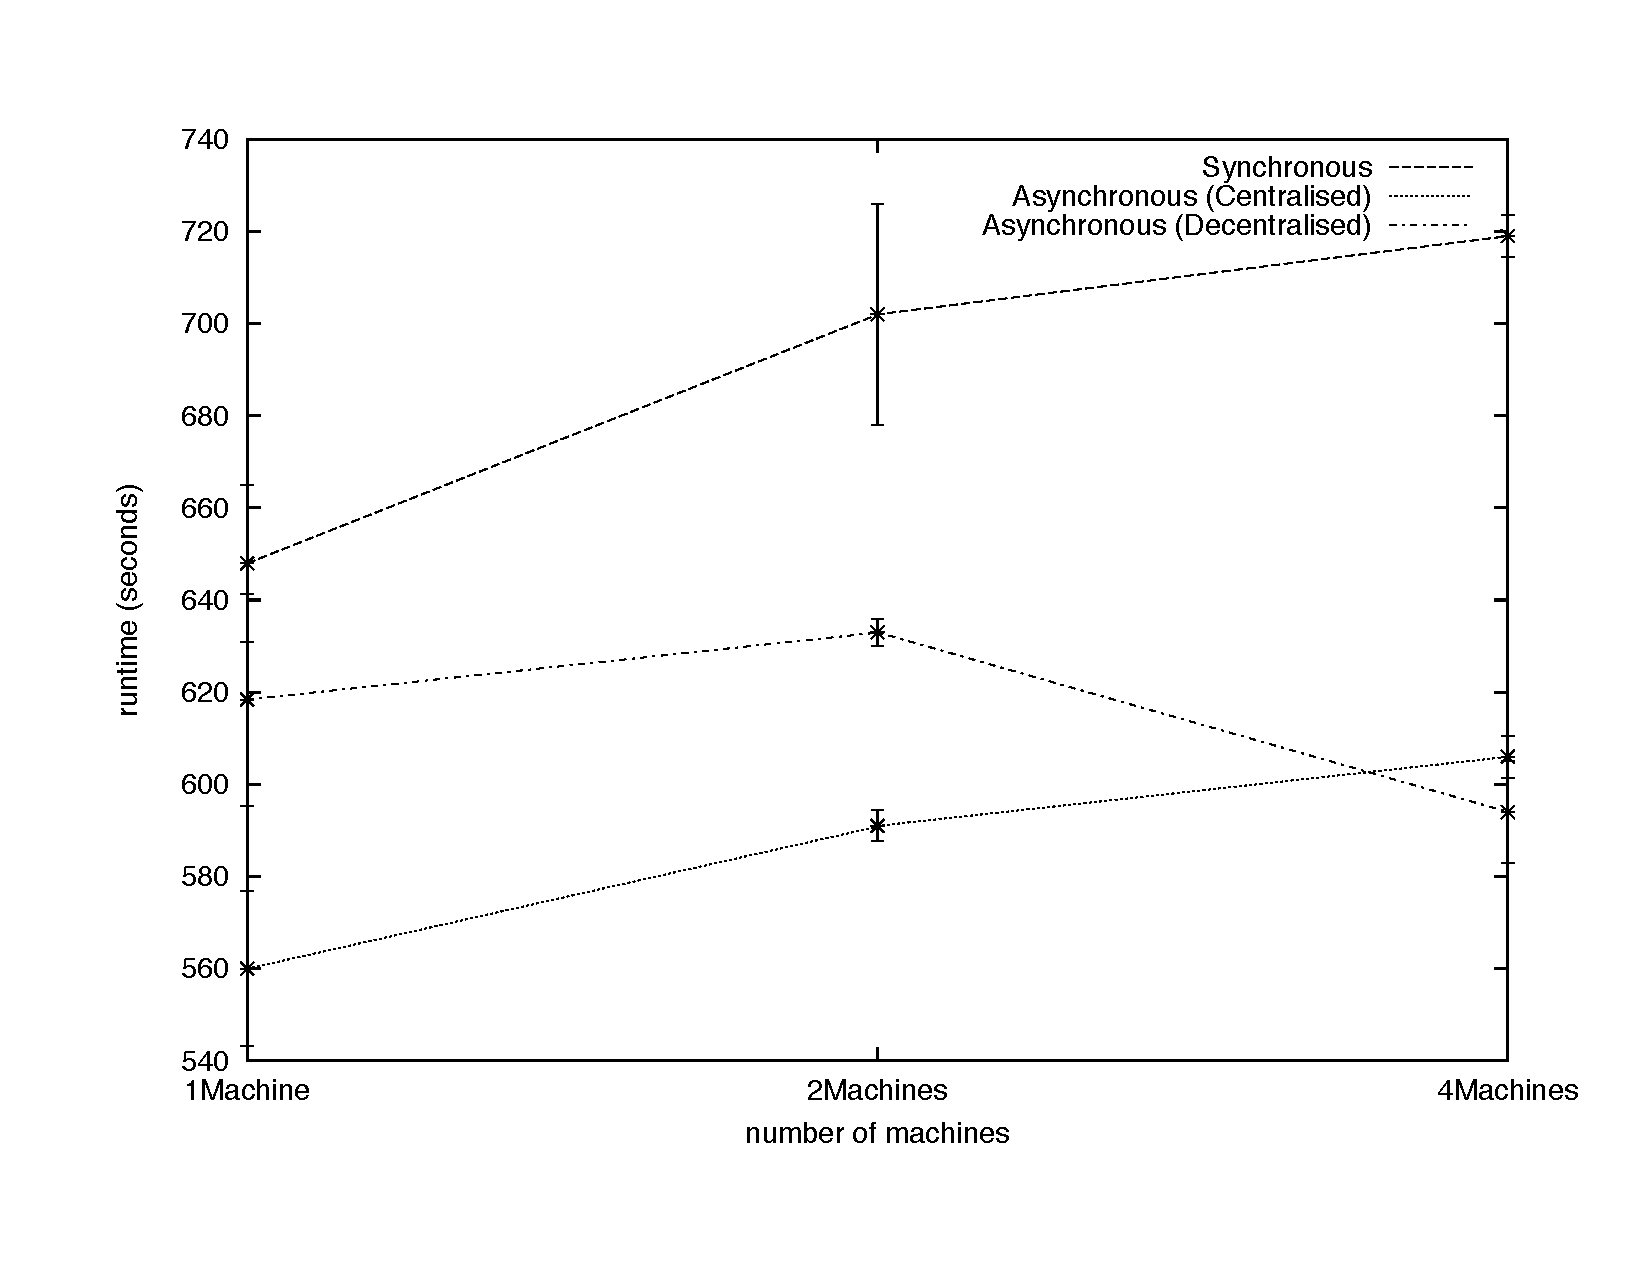
\includegraphics[width=0.47\textwidth]{../data/scaleo_16.pdf}}\\
\subfigure[32 replicas]{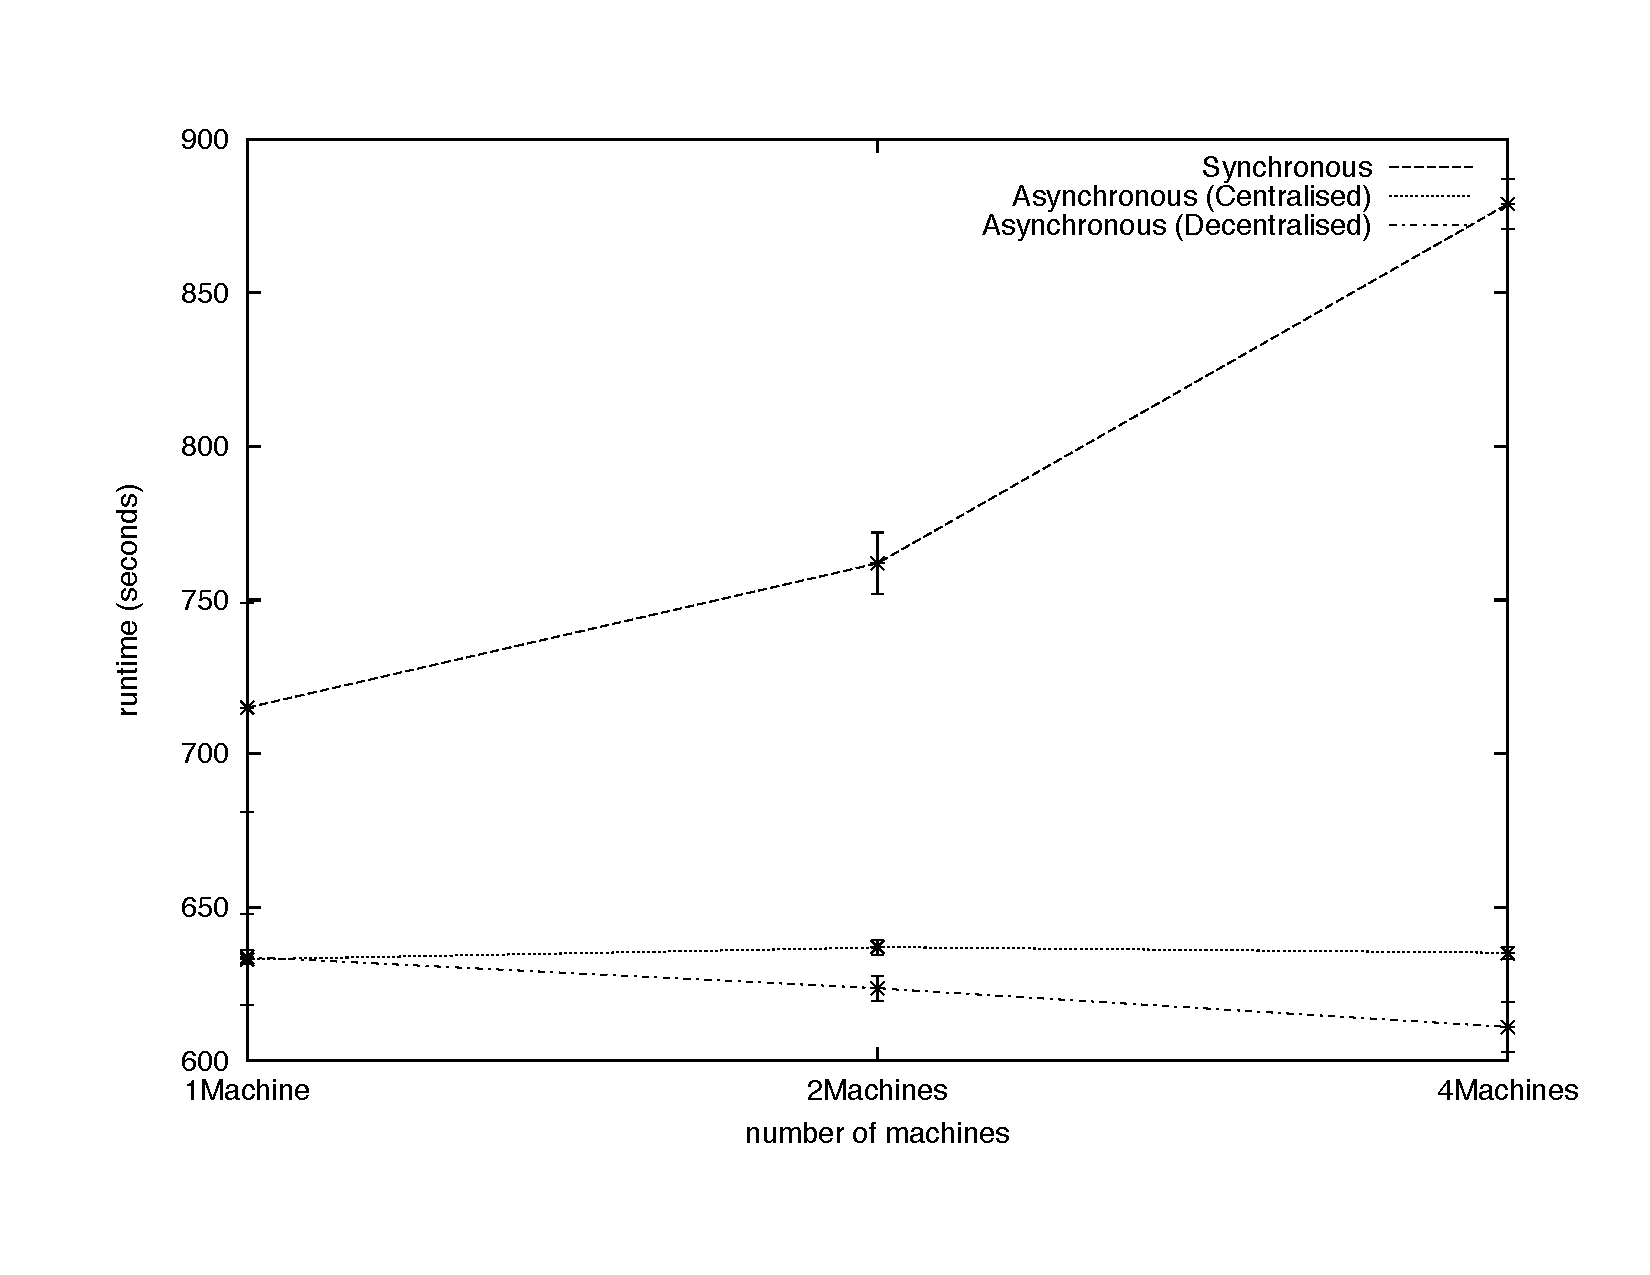
\includegraphics[width=0.47\textwidth]{../data/scaleo_32.pdf}}
\caption{\textbf{Scale-out Performance for 8, 16 and 32 Replicas:} 
  TBD.}
  \alnote{16 or 32 replicas? Why is the centralised async performing better for 8 replicas and a small number of machines? bar chart instead of lines? opinions?}
\label{fig:24machines}
\end{figure}

\subsection{Scale out}

\subsubsection{Experiments}
In this section, we describe the experiments we did while increasing
the number of machines across which the experiments were done. We
chose LONI and Teragrid machines to run the experiments. We did
experiments distributed across two and four machines with 8, 16 and 32
replicas distributed equally across the machines.
Figure~\ref{fig:24machines} shows the behaviour of the three scenarios 
across one, two and four machines,
respectively. Overall, there is not much difference between the local
and distributed runs in any case. \alnote{see comment above: Why is case II faster than III 
in the 8rep/[1,2] machine scenario?} The reason being that there is very
little interaction between the replicas. A very small configuration
file is staged to the remote machines after an exchange, which will
not add more than a couple of seconds per exchange. The rest of the
co-ordination is done via the advert service, which is usually located
on a remote machine in any case. Each query to the advert server is in
the order of milli seconds and does not produce a noticeable effect on
the performance.

\subsubsection{Scale out performance: Results and Analysis}

{\it Results:}\\


{\it Analysis: } In Figure~\ref{fig:24machines}, we see the performance
of all three cases when run in a distributed manner across two
machines. As the data that is exchanged between replicas is very
small, the Cases I, II and III behave in a similar manner to the way
they behave on a single machine. \alnote{we should add some numbers
  and maybe a graph for an example scenario: x: machines y:
  time-to-solution} Again, asynchronous RE is better suited for
distributed runs and the decentralised implementation scales best. The
reason is, since each replica has its own replica agent, there is no
need to transfer any files between machines. The required
configuration files are created locally by the replica agent.


%In Case I, the pair-wise replica exchange can occur only between replicas of the same generation. Therefore, each exchange step is attempted only after all the replicas have finished running. After the exchange, all the replicas are restarted sequentially. This inserts a delay between the start time of the first replica, the last replica and the replicas in between. %As more resources become available at different times, the replicas already running or done are forced to wait for the newly running replicas to finish before moving on to the next exchange step. %Each exchange step is counted as an exchange.
%In Case II, the pair-wise replica exchange can take place between any two replicas in the ensemble irrespective of generation. As more resources become available, the new replicas join the ensemble immediately and the replicas already running are not restrained from attempting exchanges or restarting. This gives the asynchronous or synchronous RE a slight advantage. But with a large number of replicas we could easily see large difference.
%\athotanote{Further, we show performance gains by running across more than one machine. By running across more than one machine, we demonstrate the ability to divide the jobs into smaller sub-jobs and then distribute them across a number of machines, thereby reducing the risk of long queue wait times on an over-crowded resource. In Figure~\ref{fig:graph}, it can be seen that the asynchronous RE time to completion improves almost by a factor of 3 when moving from one machine to four machines. This was caused due to the fact that when the experiment was done on one machine, by the time the experiment ended, only 64 cores were allocated by the resource manager. But on the other hand, when the experiment was launched across four machines, it received an allocation of 64 cores on each of the four resources. The improvement that is seen in the case of synchronous RE from one to four machines is also due to a similar reason.} %The asynchronous RE appears faster by a couple of minutes due to the fact that when the BigJobs become available randomly, the synchronous RE has to wait for the newly running replicas to finish.

%slightly over 2 machines, but again increases over 4 machines. This is due to the fact that the experiments have been run only a handful of times but, over time, it can be assumed that it will result in reduced queue wait times.

\section{Conclusion}
\label{sec:conclusion}


%\athotanote{is this right? }
% We are also going to have a wider group of replicas to look at for
% each replica as we are not pairing the replicas.

% Also, we have the usual advantages of using a pilot-job,
% such as reduced queue wait times by not having to submit to the queue
% at every step.  We also provide major advantages when compared to
% Parashar et al.

%  to run the asynchronous RE simulations,
% including the ability to run MPI
% jobs.
% ??We need to evaluate the performance of our models and compare with other models for conducting replica exchange simulations.


%%%%% FIGURE %%%%%
%\begin{figure}
%\centering
%\subfigure[Time to complete 64 exchanges on QB with two 64 core BigJobs and on both QB/Louie jointly with a 64 core BigJob on each machine.]{
%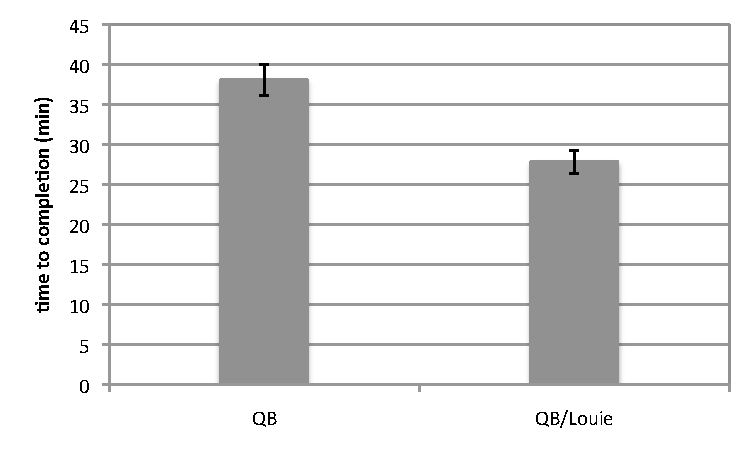
\includegraphics[width=0.40\textwidth]{figures/graph1.pdf}
%\label{fig:subfig3}
%}
%\hspace{0.5cm}
%\subfigure[Time to complete different number of exchanges on QB/Louie with a 64 core BigJob on each machine.]{
%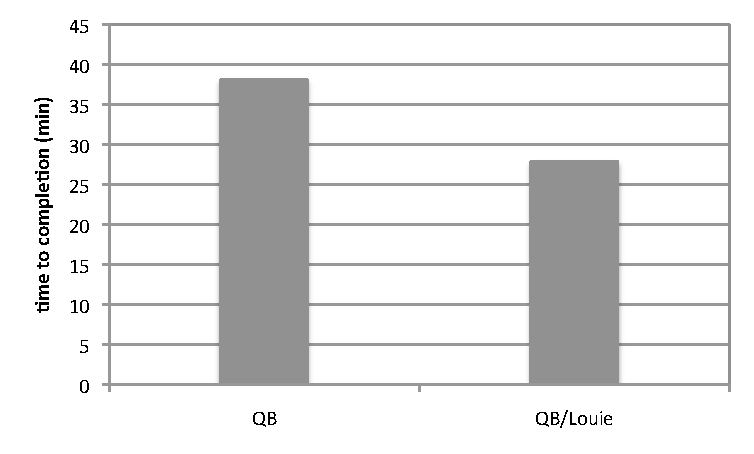
\includegraphics[width=0.40\textwidth]{figures/graph2.pdf}
%\label{fig:subfig4}
%}
%\caption{\small In Figure 2(a), we can see the improvement in performance when run on more than one machine. It is due to the fact that usually the first queued job becomes active before the second on a machine and running jobs on more than one machine solves this problem. In Figure 2(b), we can see consistent performance over prolonged runs, making 32, 64 and 128 exchanges.}
%\label{fig:graphs}
%\vspace{-1em}
%\end{figure}
%%%%% FIGURE %%%%%

An important motivation for this work is to implement a scheme that does not depend on a
static, well defined model of resource availability. %We test and scale
%our implementation on production level grids such as Teragrid and
%LONI~\citep{LONI_web}.
Preliminary results, shown in Figure~\ref{fig:graph}, indicate the
most important advantages of asynchronous RE and SAGA/BigJob over
traditional RE: (a) allows for exchanges to occur between replicas
with non-nearest temperatures, which in turn allows crosswalks to
happen (b) a reduced time to completion when running on more than one
machine due to improved resource availabilities, (c) the advantage of
using a pilot-job mechanism, which eliminates the waiting times at the
local resource manager, \alnote{have shown this in prev. papers, but
  we don't really have data in this one} and (d) the ability to scale
out across different production level infrastructure, such as, the
Teragrid and LONI.
% It performs well even after doubling and quadrupling the number of
% exchanges required to complete the simulation. The time to
% completion only increases by 35\% after doubling and 117\% after
% quadrupling the number of exchanges.
%\athotanote{should the results
%  be included in the conclusion or in a separate results section? Do
%  you agree with the \# of exchanges scheme to show the data?}
% Unfortunately we have results only for Case II currently, but 

%In summary, we have established the ability to scale-out across different
%infrastructure and compared the performance of the asynchronous
%RE with the synchronous RE at large scales. 
Further, we compare the traditional RE model (case I) and the centralised (case II) and decentralised (case III) models of the asynchronous replica exchange by modeling and repeating the experiments a reasonable number of times, so as to accurately quantify the scientific and performance gains. %We also propose to measure the frequency with which crosswalks occur with increasing number of replicas and measure the advantages due to a decentralized implementation in the full paper.


%With this asynchronous replica exchange mechanism we can improve the
%number of exchanges per unit time, a key parameter in judging the
%performance of a replica-exchange mechanism. \athotanote{is this
 % right? }  We are also going to have a wider group of replicas to
%look at for each replica as we are not pairing the replicas. Also, we
%have the usual advantages of using a pilot-job, such as reduced queue
%wait times by not having to submit to the queue.  Unfortunately we
%dont have results \jhanote{What results can we present -- any? some?},
%so we will say, (i) we establish the ability to scale-out (distributed
%and exa-scale) across different infrastructure (ii) compare the Async
%versus sync formulation at unprecedented scales \jhanote{At least
%  outline what infrastructure we / you are planning to use?} (iii)
%compare different implementations of the Async version
 

\begin{acknowledgement}
  This work is part of the Cybertools (http://cybertools .loni.org)
  project and primarily funded by NSF/LEQSF (2007-10)-CyberRII-01.
  Important funding for SAGA has been provided by the UK EPSRC grant
  number GR/D0766171/1 (via OMII-UK) and HPCOPS NSF-OCI 0710874. This
  work has also been made possible thanks to computer resources
  provided by TeraGrid TRAC TG-MCB090174 and LONI resources.
\end{acknowledgement}

\bibliographystyle{kluwer}
\bibliography{saga,literature}    
\end{document}


% and $T_W=T_w+T_r$, and where
%($T_w$), 

% \begin{eqnarray}
% T = {1\over p} \times [(T_{MD} \times  {N_X \over {N_R \over 2}}) + (T_{X} + T_{W}) \times N_X]
% \label{eq:totaltime}
% \end{eqnarray}

% \alnote{Using ex and EX as subscripts is very
%   confusing!} \jhanote{Why not use T$_X$ in lieu of $T_{EX}$? }

% Equation \ref{eq:totaltime} gives the total time to complete an RE
% experiment. The next equation aims to calculate the time to complete
% particular number of exchanges ($N_z$), where $0 \geq N_z \geq N_X$.

% \begin{eqnarray}
% T_z = {1\over p} \times [(T_{MD} \times  \lceil{N_z \over {N_R \over 2}}\rceil) + (T_{EX} + T_{W}) \times N_z]
% \label{eq:parttime}
% \end{eqnarray}

% Here $\lceil$ $\rceil$ denotes the ceiling function. The reason we put the term ${N_z \over {N_R \over 2}}$ under a ceiling function is because the ensemble of replicas run concurrently and for each concurrent run, $N_R \over 2$ exchanges are possible. Therefore, only the coordination and waiting costs effect the total time. 

% \athotanote{please suggest alternative terms if you find anything
%   confusing}

%It should be noted that only the coordination and waiting costs are divided by $\eta$. The ensemble of replicas are already running concurrently and 


% The RE algorithm involves the concurrent execution of multiple similar
% simulations, the \emph{replicas}.  There is a loose-coupling between
% the replicas in form of periodic exchange attempts between paired
% replicas. The traditional approach to RE is the synchronous model,
% which works well in an ideal scenario with a well defined model of
% resource availability. But with heterogenous systems and fluctuating
% resource availability, the asynchronous RE model could be more
% effectively used to conduct simulations. 
% >>>>>>> .r3441


%Previously, we demonstrated the usage of the SAGA Pilot-Job
%framework~\citep{saga_bigjob_condor_cloud} -- called the BigJob, to run
%RE simulations across multiple, heterogeneous distributed Grid and
%Cloud infrastructures~\citep{Luckow:2008fp}.
%\alnote{maybe we should also intro SAGA at some point} \jhanote{Yes} The Simple API for Grid Applications (SAGA)~\citep{saga_gfd90} is an API standardization effort within the Open Grid Forum (OGF)~\citep{ogf_web}, an international standards development body concerned primarily with standards for distributed computing. The various tasks that are carried out using the SAGA APIs include file staging, job spawning and the conduction of the exchange attempts.
%Further, we introduced several adaptivity modes, e.\,g.\ adaptive
%sampling that are able to react to dynamic changes in resource
%availabilities.

%\alnote{Not sure how many technical we need to provide...}  

%Traditionally, depending
%on the number of processes \texttt{N}, the manager creates \texttt{N/2} pairs
%of replicas.  Before launching a job, the manager ensures that all
%required input files are transferred to the respective resource. For
%this purpose, the SAGA File API and the GridFTP adaptor are used. The
%replica jobs are then submitted to the resource using the SAGA CPR
%API and the MIGOL/GRAM middleware.

%\jhanote{Mention that these are SAGA-based implementations. Something  else would be implemented differently}
%\alnote{Proposed structure: a) math. model b) sync c) async. We should give the reader some orientation in this section.}
% \jhanote{Abhinav: I still note the inconsistent and variable use of
%   algorithms, methods(?) and cases/approaches. I think we should refer
%   to Replica-Exchange as a ``class of algorithms'' or ``algorithm'',
%   and different implementations -- sync versus async} 

% \athotanote{RE class of algorithms - synchronous and asynchronous
%   models within RE class of algorithms; later sync, centralized-async,
%   decent-async implementation. right? or - RE class of algorithms -
%   synchronous and asynchronous implementation of RE class of
%   algorithms; later sync, centralized-async, decent-async
%   implementations. please suggest.}  \jhanote{I would say (i) RE Class
%   of Algorithms, (ii) Sync/Async algorithms too, and then centralized
%   or decentralized implementations of these sync versus async RE
%   algorithm}
%\subsection{Mathematical Model}
%\alnote{I think we should discuss the mathematical model before going
%  into the specifics of sync/async RE.}
%Here we first provide a basic mathematical model for different RE
% models which explains the terms involved. In this section, we aim to
% develop an equation for total time to run any RE simulation. If $t$
% is the average time between successful exchanges, and $p$ is the
% probability of a successful exchange,
%\begin{eqnarray}
%t=  {1 \over p} \times {[T_{MD} + T_{X} + T_{W}]} 
%\label{eq:timebtw}
%\end{eqnarray}
%where $T_{X}$ is the time to carry-out a pairwise exchange, which is
%comprised of (i) finding a partner, (ii) exchanging states including
%file transfer, (iii) book-keeping, and (iv) (re)starting the replica;
%$T_{W}$ is the time spent waiting for all replicas to complete running.
%Therefore, ${T_{X}} = {T_F + T_{ex} + T_{coord}}$ 
%and for ${T_{X}}^{async}, T_W = 0$
%The time ($T$) for N$_{X}$ exchanges is therefore $N_{X} \times t$
%If there are $\eta$ independent exchange events occurring
%concurrently, then the time $T$ for N$_x$ exchanges is $T \over \eta$.
